\chapter{EPR Spectroscopy of TEMPO-Salen Electrochemical Cells}
Here the EPR spectra of TEMPO-Salen electrochemical cells are shown under operating conditions and ex situ, for various states of charge, as well as the spectra of the materials that were used to construct the cells.
That information is used to decompose the complex spectra of a charging cell and to perform its quantitative analysis to identify the state of charge of the cell and the by-products that are being released during the cell operation.

\section{cwEPR Spectroscopy of TEMPO Containing Molecular Fragments}
% todo: the reader knows about TEMPO, dits and ditbus. Show how they behave in cwEPR spectrometer.
% picture of molecule - spectrum - diagram
The stable TEMPO$^\bullet$ radical is widely used in the EPR spectroscopy as a spin probe and particularly in the EPR studies of TEMPO containing ORB materials~\cite{nakahara2002_cpl, nishide2004_electact, bahaceci2013_jpowersources, aydin2015_jsoistatelect, khodeir2019_softmatter, Zhang2018}. The spin density at the TEMPO$^\bullet$ radical is localized within the N-O bond~\cite{Owenius2001} and partially resides on the $I=1$ $^{14}$N nucleus, so to describe the EPR spectrum of an isolated TEMPO$^\bullet$ one has to take into consideration the electron Zeeman term $H_{EZ}$, the nuclear Zeeman term $H_{NZ}$ and the hyperfine coupling term $H_{HF}$. The unpaired electron spin on TEMPO$^\bullet$ has anisotropic g value, because of the asymmetry of its molecular orbital, so the $\textbf{g}$ matrix and the $\textbf{A}$ hyperfine coupling tensor are both anisotropic. $\textbf{g}$ is diagonal in the molecular frame of reference shown in Figure~\ref{fig:TEMPO_dft}. Its principal values are $\left[g_{xx}=2.009,g_{yy}=2.006,g_{zz}=2.002\right]$~\cite{Liu_2008,Bordignon2017}. The principal values of $\textbf{A}$ in the same frame are $\left[A_{xx}=20,A_{yy}=20,A_{zz}=100\right]$~MHz~\cite{Liu_2008,Bordignon2017}.


\begin{figure}[h]
\center
	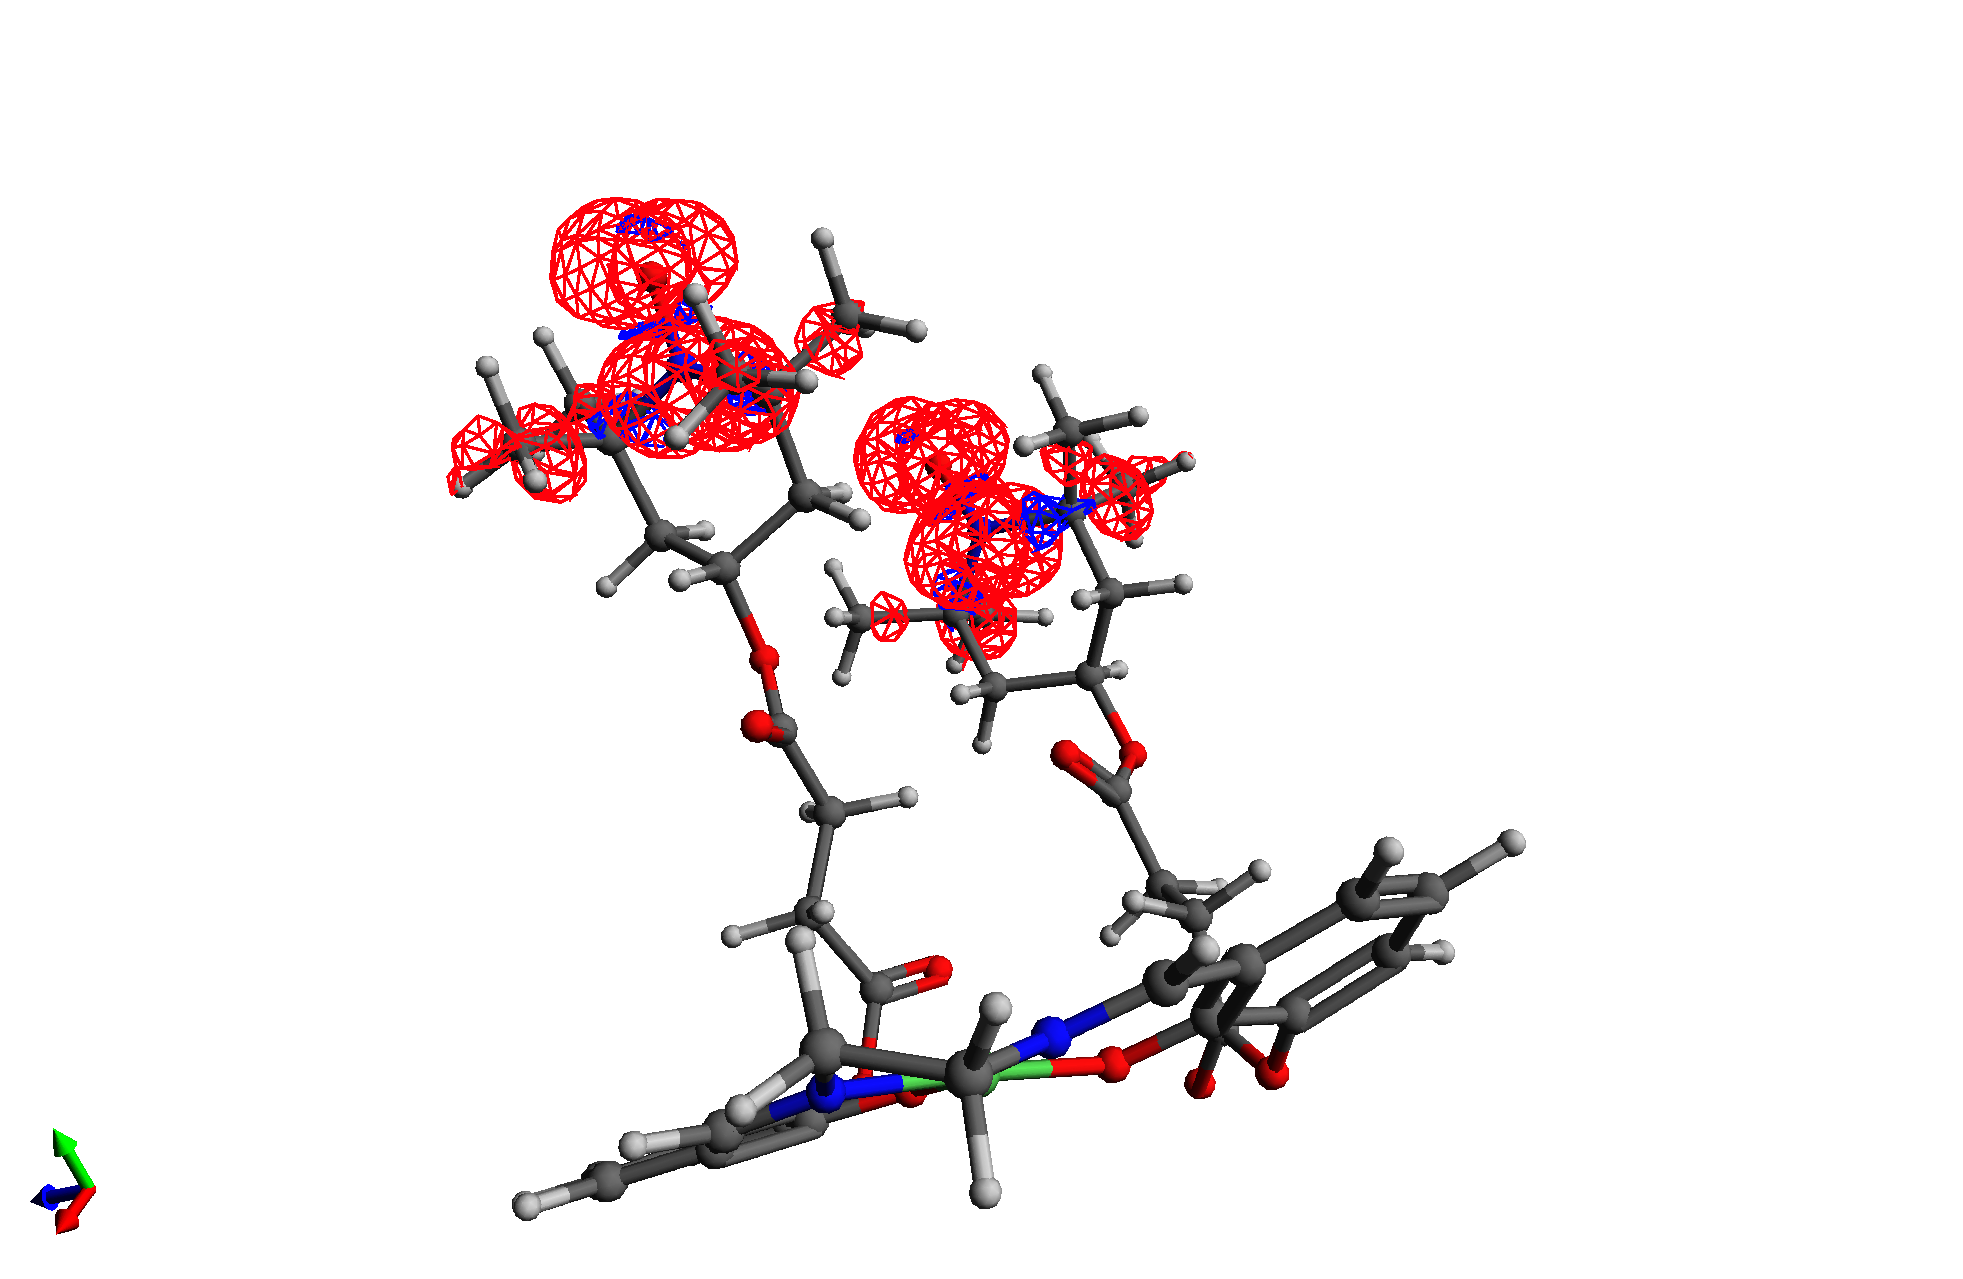
\includegraphics[width=1\textwidth]{./operando_epr/figures/DITS_DFT.pdf}
	\caption{DFT on DiTS showing spin density on two neighboring TEMPO groups. The spin density is localized around the Nitrogen nucleus that gives rise to the hyperfine coupling. Calculation by Marcel Gauglitz.}
	\label{fig:TEMPO_dft}
\end{figure}



\subsection{Room Temperature Spectra of TEMPO$^{\bullet}$ Solutions}
Solution spectra of radicals are showing averaged values of $g$ and $A$ because of the fast molecular tumbling~\cite{Liu_2008,Carrington_solution_epr}. The observed $g$ value for a tumbling TEMPO$^{\bullet}$ is the average of the principal values of the $\textbf{g}$ matrix: $g = 1/3\left(g_{xx}+g_{yy}+g_{zz}\right)$. The anisotropic part of the hyperfine coupling tensor for the tumbling TEMPO$^{\bullet}$ also averages to zero, so only the isotropic hyperfine constant $a_{iso}$ determines the observed hyperfine coupling. CwEPR spectra of a 0.1~mM solution of TEMPOL measured at room temperature are shown in Figure~\ref{fig:cwEPR_monoTEMPO_diTEMPO}. The spectral simulation performed with EasySpin~\cite{Stoll2006} yields $g=2.0055$ and $a_{iso}=43.8$~MHz.

\begin{figure}[h]
\center
	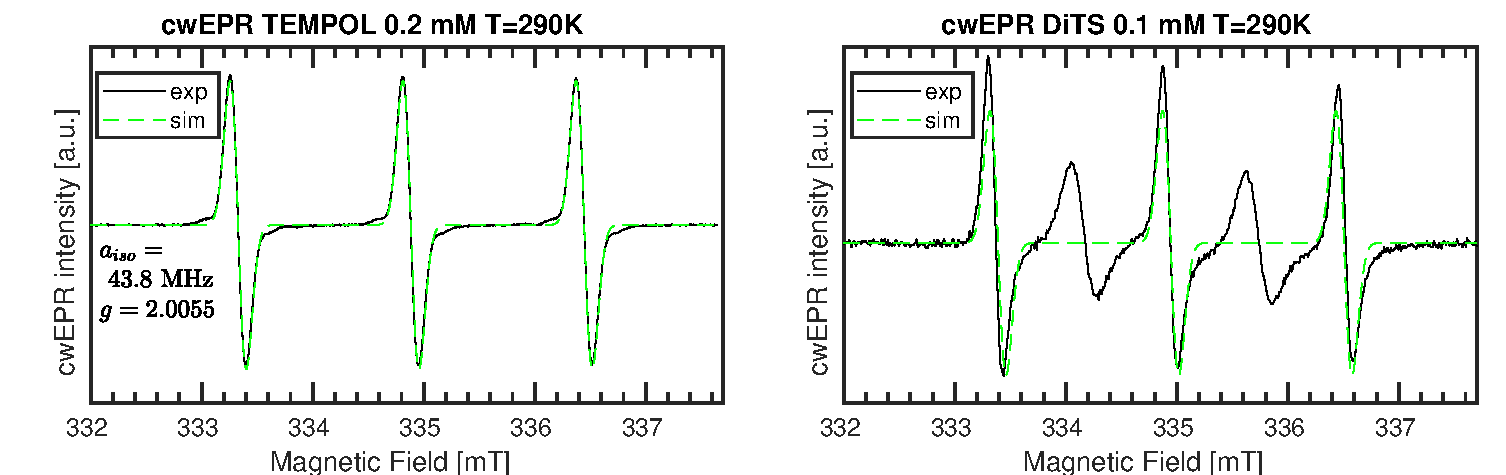
\includegraphics[width=1\textwidth]{./operando_epr/figures/TEMPOL/cwEPR_TEMPOL_vs_DiTS_RT.pdf}
	\caption{Room temperature cwEPR spectra of a low-concentration solutions containing mono- and di-TEMPO molecular fragments. Left: TEMPOL, Right: Di-Tempo-Salen.}
	\label{fig:cwEPR_monoTEMPO_diTEMPO_SOLUTION}
\end{figure}
\begin{figure}[h]
\center
	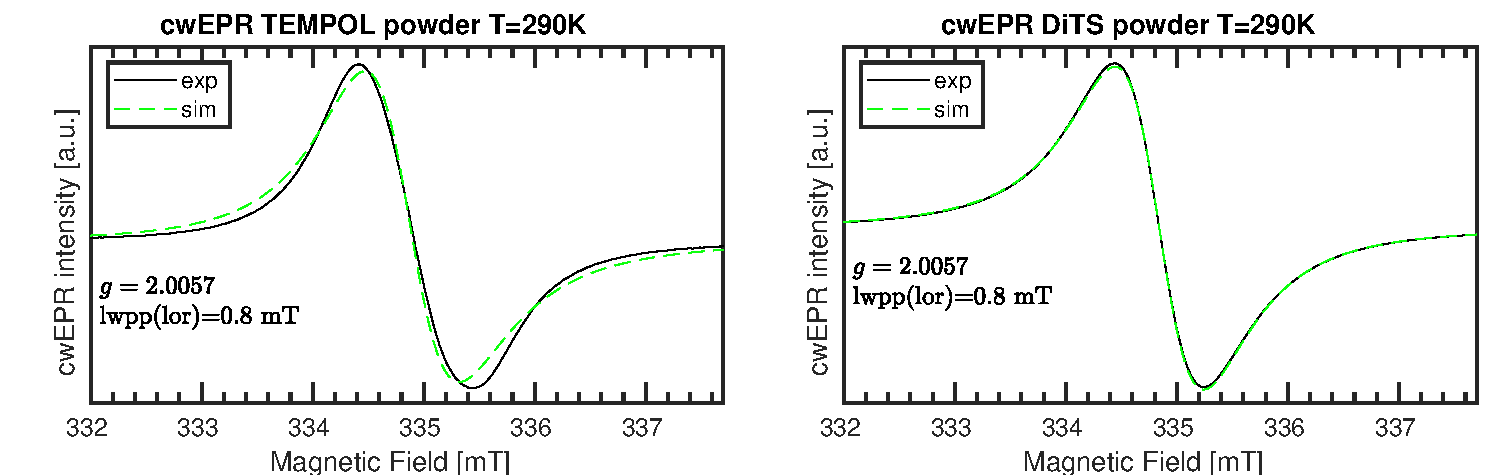
\includegraphics[width=1\textwidth]{./operando_epr/figures/TEMPOL/cwEPR_TEMPOL_vs_DiTS_RT_POWDER.pdf}
	\caption{Room temperature cwEPR spectra of pure TEMPO-containing powders. Left: TEMPO, Right: Di-Tempo-Salen.}
	\label{fig:cwEPR_monoTEMPO_diTEMPO_POWDER}
\end{figure}

\begin{figure}[h]
\center
	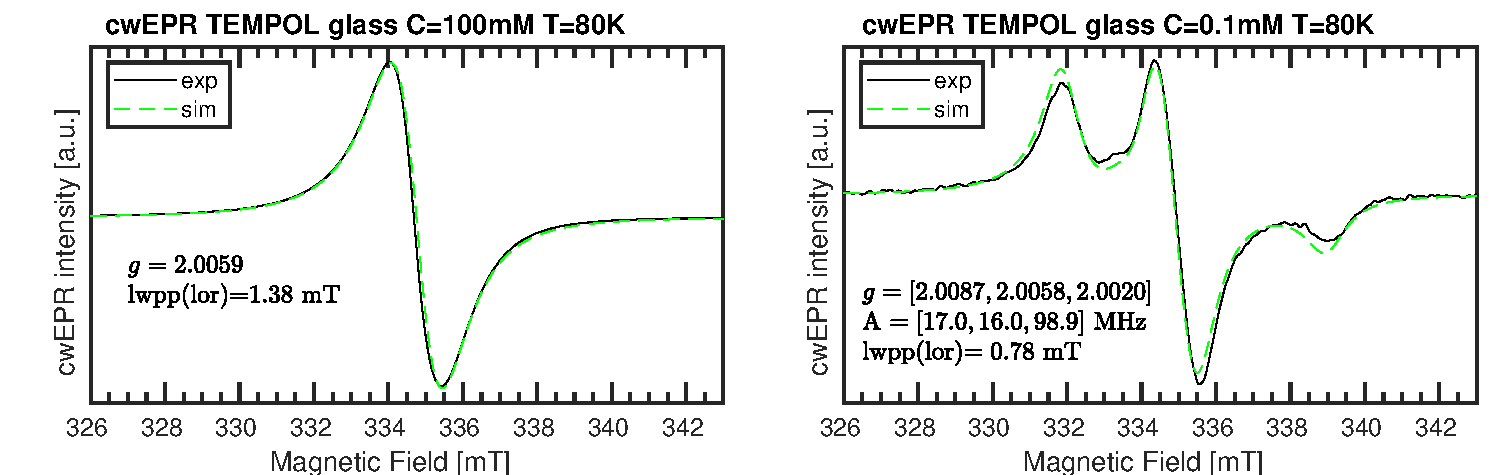
\includegraphics[width=1\textwidth]{./operando_epr/figures/TEMPOL/cwEPR_TEMPOL_100mM_vs_p1mM_80K.pdf}
	\caption{Cryogenic cwEPR spectra of TEMPOL at high and low concentration in a Dichloroethane/Acetonitrile glass. Left: 100~mM, Right: 0.1~mM.}
	\label{fig:cwEPR_TEMPOL_High_Low_Concentrations}
\end{figure}



\par
A biradical molecule like Di-Tempo-Salen (Figure~\ref{fig:molecules} e) and f)) has two paramagnetic species that are close to each other and therefore exchange electrons. When the exchange coupling between the radicals $J$ is comparable to the hyperfine coupling $A$ of each radical to its 'host' nucleus, the superhyperfine interaction~\cite{} takes place, in which the radical is interacting to the nucleus of the neighboring radical~\cite{Eaton2018}. Solutions of biradical molecules with magnetic nuclei show more features in cwEPR spectra when the electron-electron exchange coupling $J$ between the two radicals within the molecule becomes comparable to the hyperfine coupling between the radical and its 'host' $^{14}$N nucleus. tumbling of the molecule and the restricted motions of each radical within the molecule cause a complex molecular motion that affects the dipolar and exchange couplings between the radicals and causes "spectra with alternating linewidths"~\cite{Eaton2018,Carrington_g_factor}. A solution of Di-TEMPO-Salen shows a five-line cwEPR spectrum with alternating linewidhts (Figure~\ref{fig:cwEPR_monoTEMPO_diTEMPO_SOLUTION}, right) with the three most intense lines corresponding to the three hyperfine sublevels of TEMPO$^{\bullet}$. The five-line structure in the cwEPR spectrum indicates the presence of a di-TEMPO biradical in the solution.




\par
TOLYAN:\\
If the TEMPO groups are far away from each other, their cw-EPR signal consists of three
lines that are due to the hyperfine interaction between the electron spin and the spin of the Nitrogen
nucleus. When the TEMPO groups are brought closer to each other, their electron orbitals start to
overlap, and the exchange interaction (J) between the electrons grows. That splits the signal into
more lines as it was shown by [10] and represented in Fig. 7. In the case of strong exchange
interaction the spectrum consists of five lines with relative ratios 1:2:3:2:1. In the absence of the
exchange interaction the spectrum contains only three hyperfine lines of equal intensities.
In DiTS, a sum of a three-line spectrum and a five-line spectrum was observed. This may
be the evidence that TEMPO-bearing linkers are sufficiently long to allow TEMPO groups to move
freely in space around the organometallic complex. That can yield to different J values depending
on the relative orientation of the linkers, similar to [10]. In theory, there are several possible
positions of TEMPO groups relative to each other that can change the EPR spectrum. Depending
on the angle between the linkers (from $\pi$ to 0), J may vary from its minimal to maximal value,
that should yield a three- and five-line structures respectively. Since the process of movement is
dynamic, we can explain the observed picture as a combination of several positions in space [10].
The five-line structure suggests different preferred conformations of the TEMPO fragments and
dynamic interconversion between these states with different exchange coupling J leads to the
observed spectrum.

\subsection{Spectra of TEMPO$^{\bullet}$/TEMPO$^{+}$ Films}
A film made of a TEMPO-containing polymer can be brought to a certain oxidation state, depending on how many of the TEMPO groups are in the radical (TEMPO$^{\bullet}$) state and how many are in the oxidized (TEMPO$^{+}$) state. The densely packed TEMPO$^{\bullet}$ fragments in the film cannot be considered as isolated molecules anymore, and the interactions between the radicals become significant. Microcrystals of TEMPOL are densely packed TEMPO$^{\bullet}$ with a concentration of $???$~mM. The cwEPR spectrum of TEMPOL microcrystals in Figure~\ref{fig:cwEPR_monoTEMPO_diTEMPO_POWDER, left} is one broad line centered at $g=2.0055$. A powder of DiTS monomers is showing the same cwEPR spectrum in Figure~\ref{fig:cwEPR_monoTEMPO_diTEMPO_POWDER, right}. It is the matter of concentration of the peramagnetic TEMPO fragments that changes the cwEPR spectral shape. In Figure~\ref{fig:cwEPR_TEMPOL_High_Low_Concentrations, left} cryogenic (80~K) cwEPR spectrum of a 100~mM solution of TEMPOL in Dichloroethane/Acetonitrile is presented. With a slight shift in $g$ factor due to the polar molecular environment of the frozen solvent~\cite{Siavash} and a broader lineshape due to a weaker exchange narrowing, the spectrum consists on one dipolar-broadened Lorentzian line. In contrast, when the concentration of the solution is lowered to 0.1~mM (Figure~\ref{fig:cwEPR_TEMPOL_High_Low_Concentrations, right}) - the inter-molecular interactions become weak enough to resolve the $A$ and $g$ anisotropy of the nitroxide radical, so the spectrum consists of three lines that can be simulated with the known $A$ and $g$ parameters.\\
A redox-active film containing TEMPO radicals, like the TEMPO-Salen cathode film, shows different cwEPR signatures depending on its redox state. Figure~\ref{fig:cwEPR_CRYO_DiTBuS_DCG_vs_CHG} represents two crypogenic cwEPR spectra of a $d\approx2$~\SI{2}{\micro\meter} DiTBuS cathode film that was discharged to $E=-50$~mV and charged to $E=+900$~mV vs. the Ag/AgNO$_3$ RE as described in Section~\ref{sec:echem_charging}. The spectral intensities were normalized to represent the signal shape not the magnitude. The discharged film shows one broad cwEPR line in Figure~\ref{fig:cwEPR_CRYO_DiTBuS_DCG_vs_CHG}, left, that reflects on the strong interactions between the non-oxidized TEMPO$^{\bullet}$ in the discharged cathode. The linewidth of the discharged film spectrum is smaller than the linewidth of the DiTS monomer spectrum, suggesting a smaller exchange interaction between the TEMPO fragments in the film~\cite{Vereshchagin2020}.\\
The oxidized film in Figure~\ref{fig:cwEPR_TEMPOL_High_Low_Concentrations}, right, shows a well resolved spectrum of an isolated nitroxide, similar to the low-concentrated solution of TEMPOL (Figure~\ref{fig:cwEPR_TEMPOL_High_Low_Concentrations, right}). A series of powers was recorded for both redox states of the film to observe possible microwave saturation effects that are crucial for the pulsed EPR experiments discussed in Chapter~\ref{ch:pulsed_epr}.

\begin{figure}[!ht]
\center
	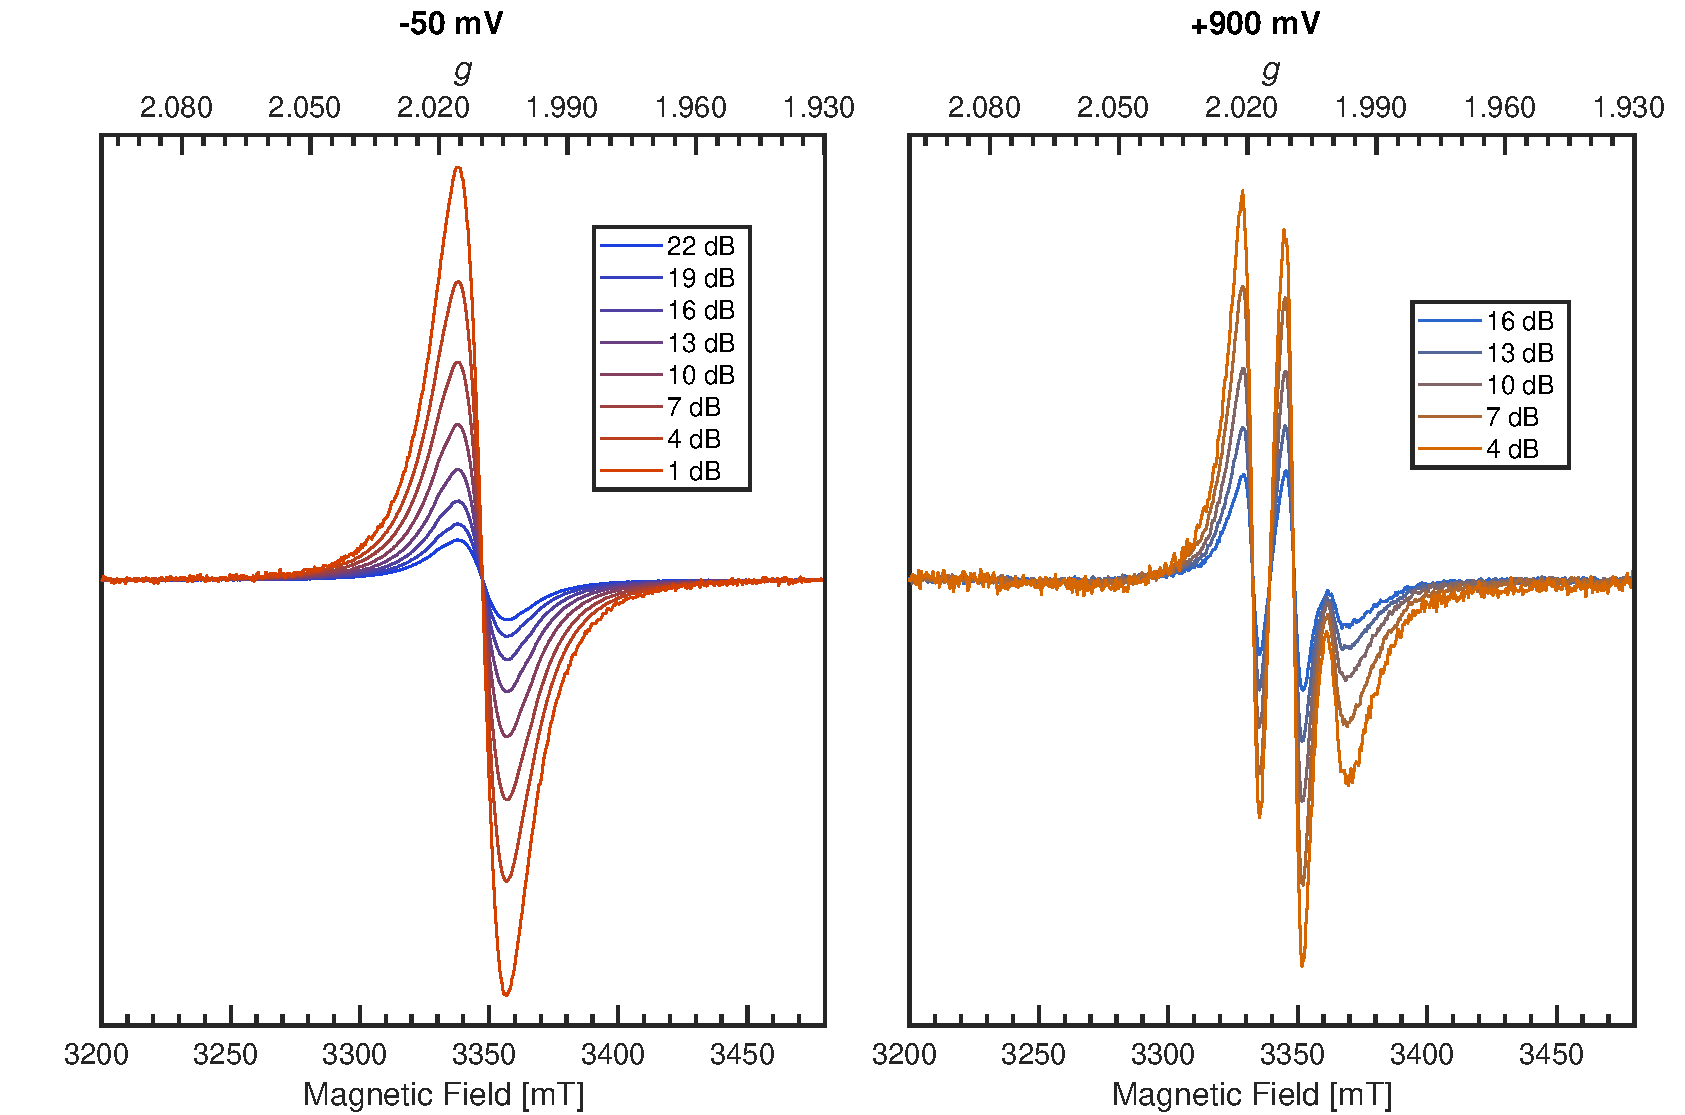
\includegraphics[width=1\textwidth]{./operando_epr/figures/CRYO/S220104_CW.pdf}
	\caption{Cryogenic (80~K) cwEPR spectra of a pDiTBuS film grown with 200 deposition cycles. Left: discharged film, -50~mV vs. Ag/AgNO$_3$ RE. Right: Fully charged film, 900~mV vs. Ag/AgNO$_3$ RE.}
	\label{fig:cwEPR_CRYO_DiTBuS_DCG_vs_CHG}
\end{figure}

\begin{figure}[h]
\center
	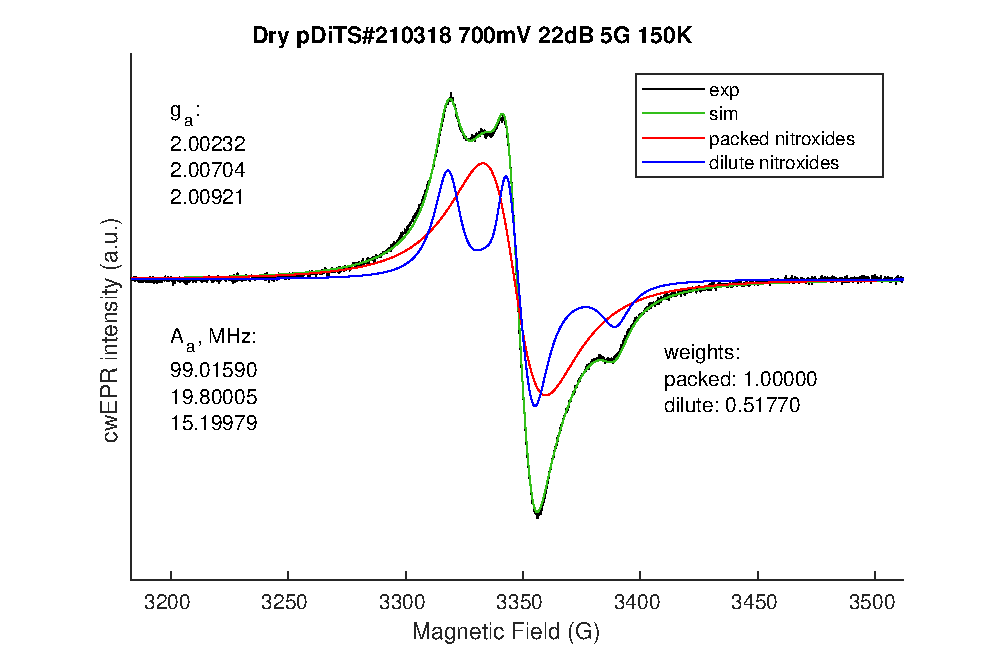
\includegraphics[width=1\textwidth]{./operando_epr/figures/CRYO/cw_sim_pDiTS_210318_700mV_2comp.pdf}
	\caption{A pDiTS film in the intermediate state of charge (700~mV vs. Ag/AgNO$_3$) showing a composition of two spectral signatures. The single-line signal from the densely packed nitroxide radicals coexists with the signal of the isolated nitroxide radicals. Two-component simulation.}
	\label{fig:cwEPR_CRYO_DiTS_2_COMP_SIM}
\end{figure}


\begin{figure}[h]
\center
	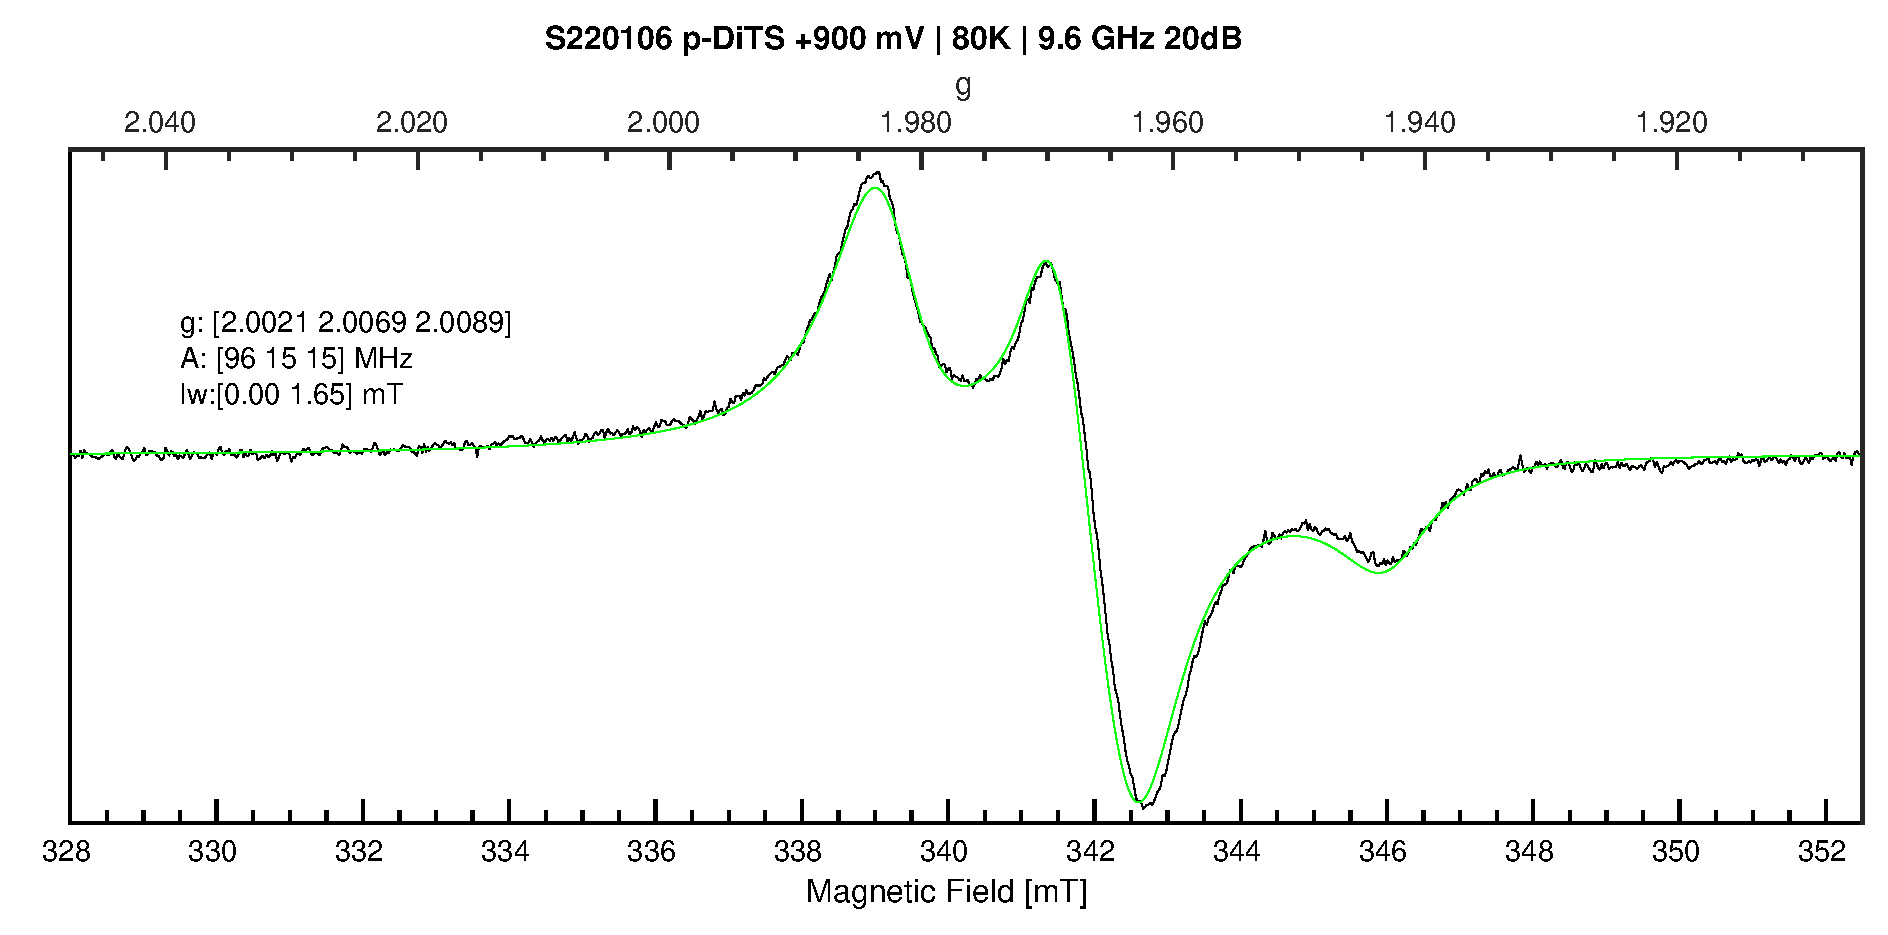
\includegraphics[width=1\textwidth]{./operando_epr/figures/CRYO/S220106_p-DiTS_OX_80K_CW_SIM.pdf}
	\caption{Cryogenic (80~K) cwEPR spectrum of an oxidized pDiTBuS film grown with 200 deposition cycles showing a signature of the isolated nitroxide radical with the standard $g$ and $A$ parameters, revealed with a simulation.}
	\label{fig:cwEPR_CRYO_DiTBuS_CHG_SIM}
\end{figure}



\begin{figure}[h]
\center
	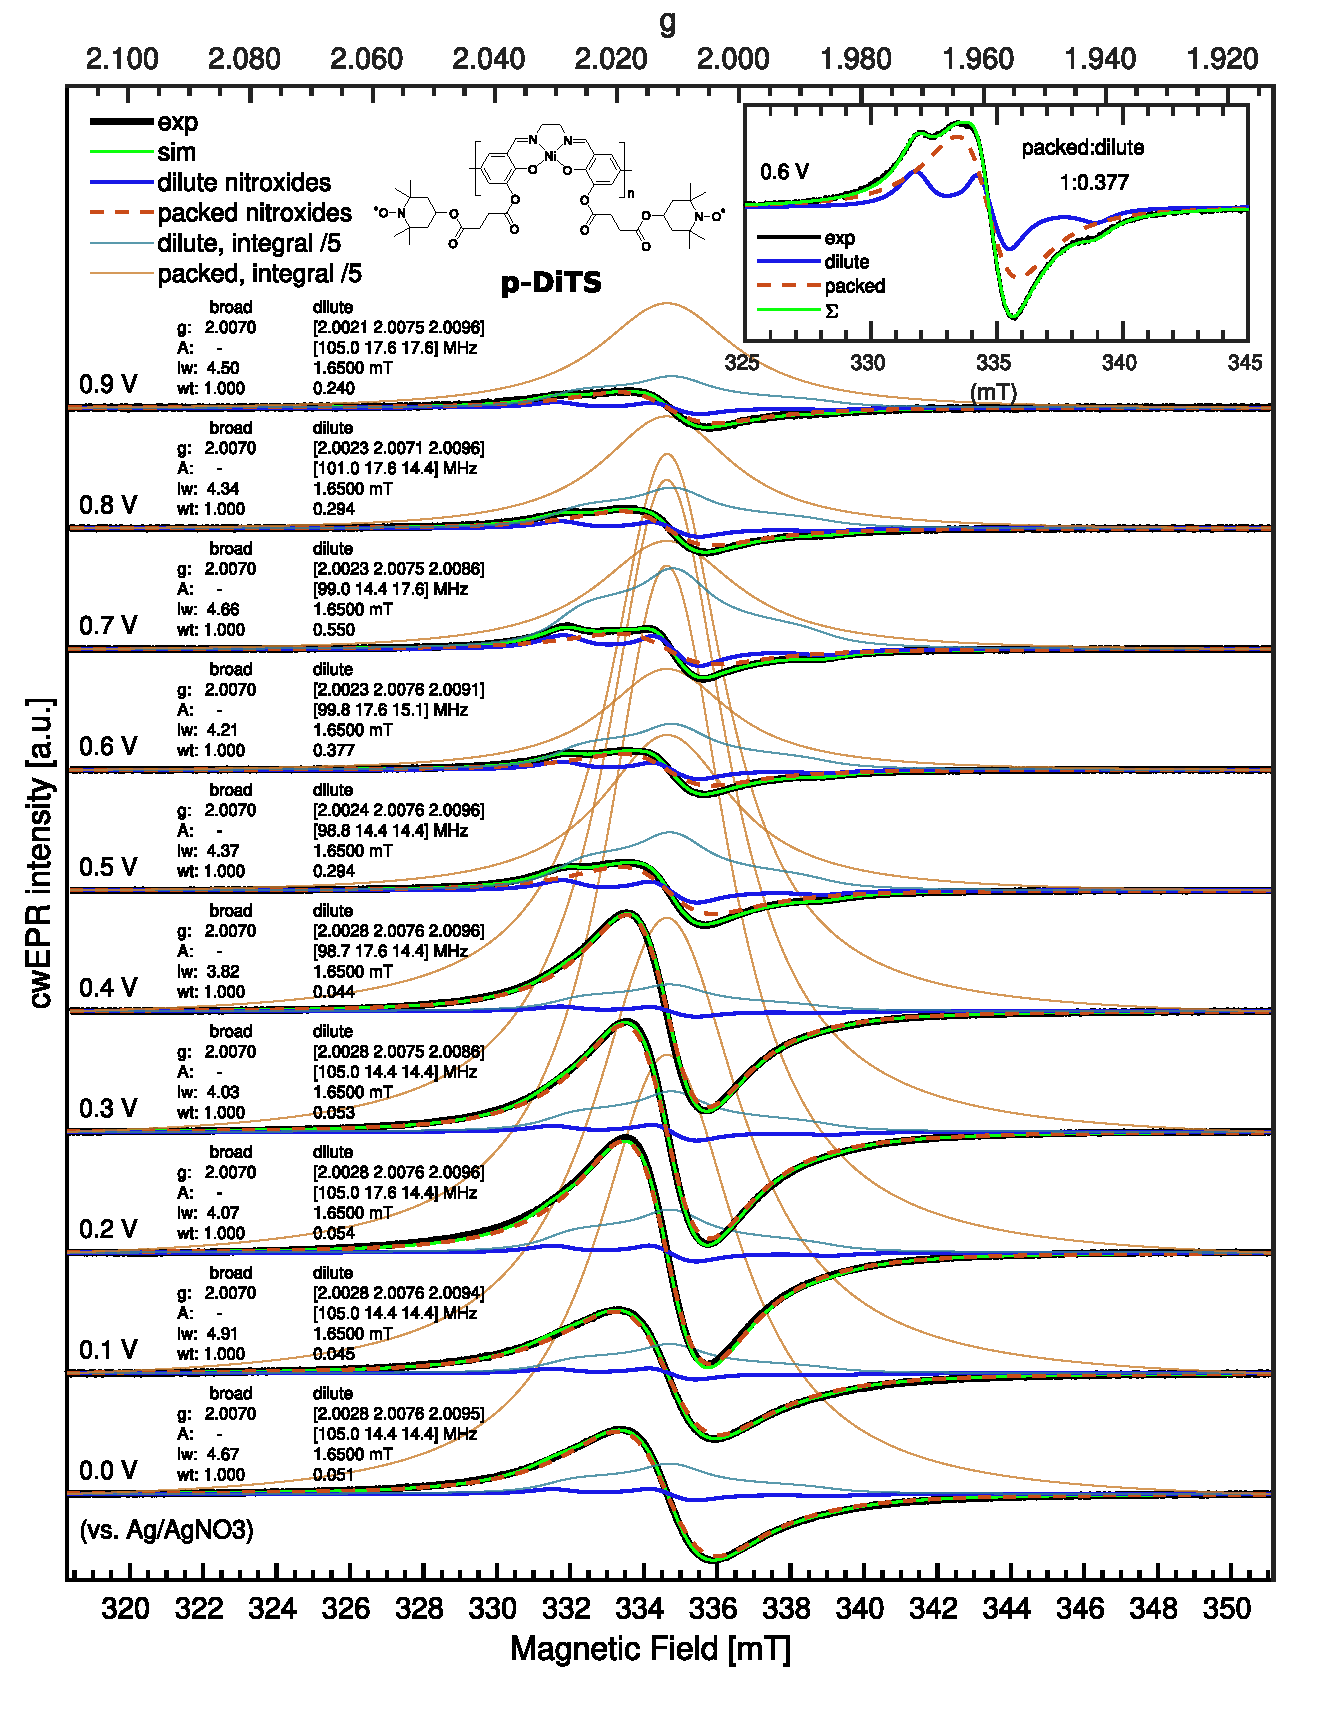
\includegraphics[width=1\textwidth]{./operando_epr/figures/CRYO/Figure_S7_new.pdf}
	\caption{Ex-situ SEC cwEPR measurements ($\nu=$9.4~GHz) on a dry p-DiTS film at 150~K. Decomposition of spectra into two components with numeric simulations using EasySpin~\cite{Stoll_2006}: a broad Lorentzian line (g = 2.0070, lw = 4.63$\pm$1.00~mT) and a dilute component with a hyperfine coupling to $^{14}$N ($I$ = 1, $g$ = [2.00231 2.00711 2.00912], $A$ = [100 15 15]$\pm$5 2 2]~MHz, Lorentzian broadening with lw = 1.65~mT). The absorption profiles are shown with the integrals of the EPR signals. The ratio between the simulated components for each potential is shown by the double integrals of the components. Inset: sum of the broad and dilute components that reproduce the line shape at 0.6~V.\\}
	\label{fig:cwEPR_CRYO_DiTS_CHG_SIM}
\end{figure}



\subsection{Spectra of NiSalen Films}
The molecular backbone of pDiTS and pDiTBuS is the pNiSalen, a conjugated polymer that exhibits redox behavior~\cite{Dmitrieva2018,Vereshchagin2020,Apraksin2021}. The observations of electrochromicity of pNiSalen films with UV-VIS spectroscopy~\cite{Dmitrieva2018} have revealed the formation of polarons and antiferromagnetically coupled (with total spin S=0) bipolarons in the oxidized state of pNiSalen. A series of cwEPR spectra recorded for a pNiSalen film in various redox states is shown in Figure~\ref{fig:cwEPR_CRYO_NiSalen_REDOX_SIM}. Operando cwEPR spectra of a cell containing a pNiSalen cathode is shown in Figure~\ref{fig:cwEPR_RT_NiSalen_OPERANDO}.

\begin{figure}[!h]
\center
	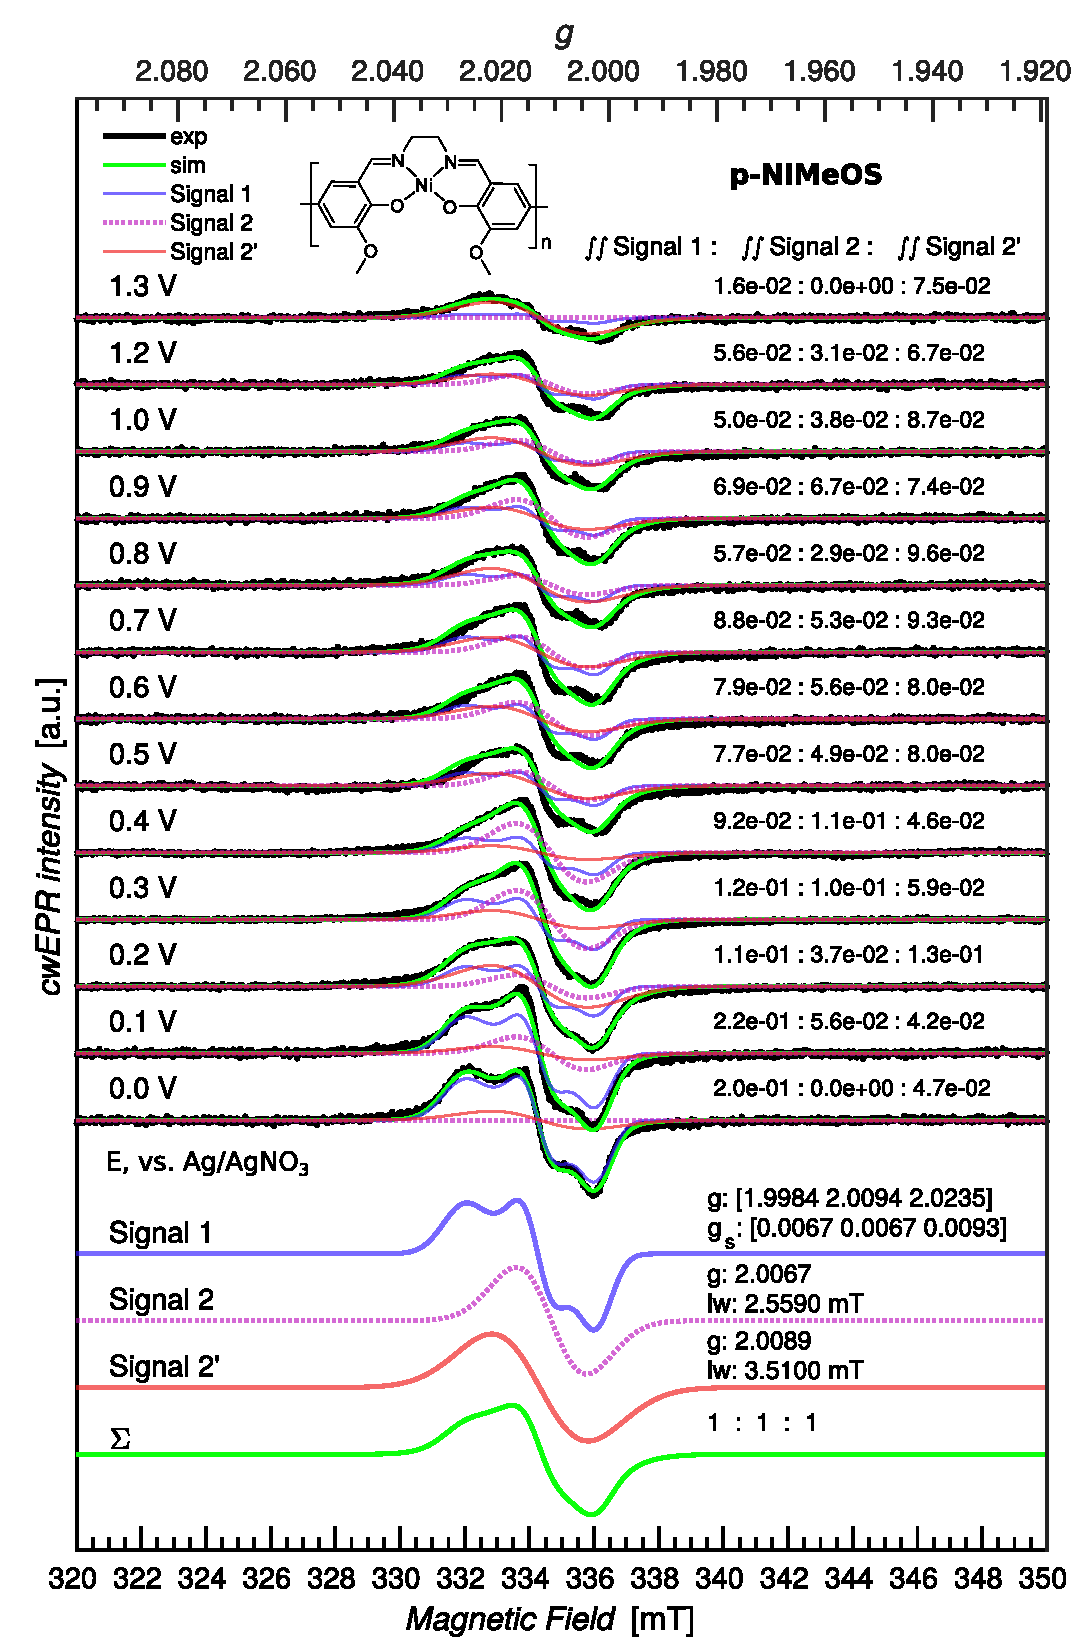
\includegraphics[width=1\textwidth]{./operando_epr/figures/CRYO/Figure_S8.pdf}
	\caption{Potential-dependent cwEPR spectra of a NiMeOSalen film measured at 150~K. Simulation of the spectra with three components reported by the Timonov group.}
	\label{fig:cwEPR_CRYO_NiSalen_REDOX_SIM}
\end{figure}

\begin{figure}[!ht]
\center
	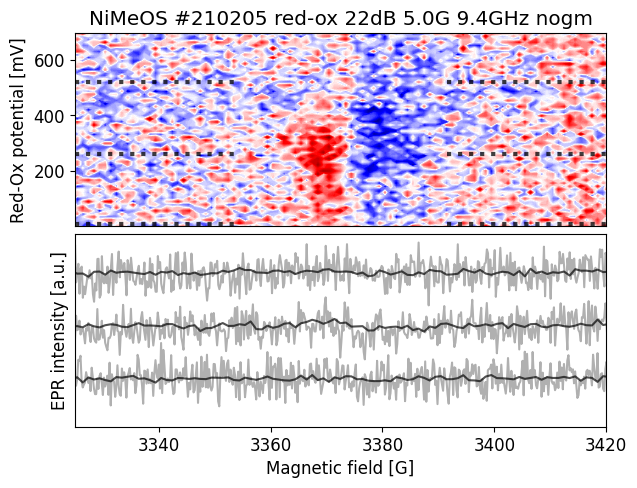
\includegraphics[width=0.6\textwidth]{./operando_epr/figures/backbone/NiMeOS_lyra_overnight_RT.png}
	\caption{Potential-dependent operando cwEPR spectra of a NiMeOSalen cathode film measured at room temperature.}
	\label{fig:cwEPR_RT_NiSalen_OPERANDO}
\end{figure}


\section{Electrochemical Cells for EPR spectroscopy}
\label{sec:operando_cell_fab}

\subsection{Cells Based on a Modified EPR Sample Tube}
\label{sec:tube_cell}
An electrochemical cell was constructed inside an X band EPR sample tube.
\begin{figure*}[ht]
 \centering
 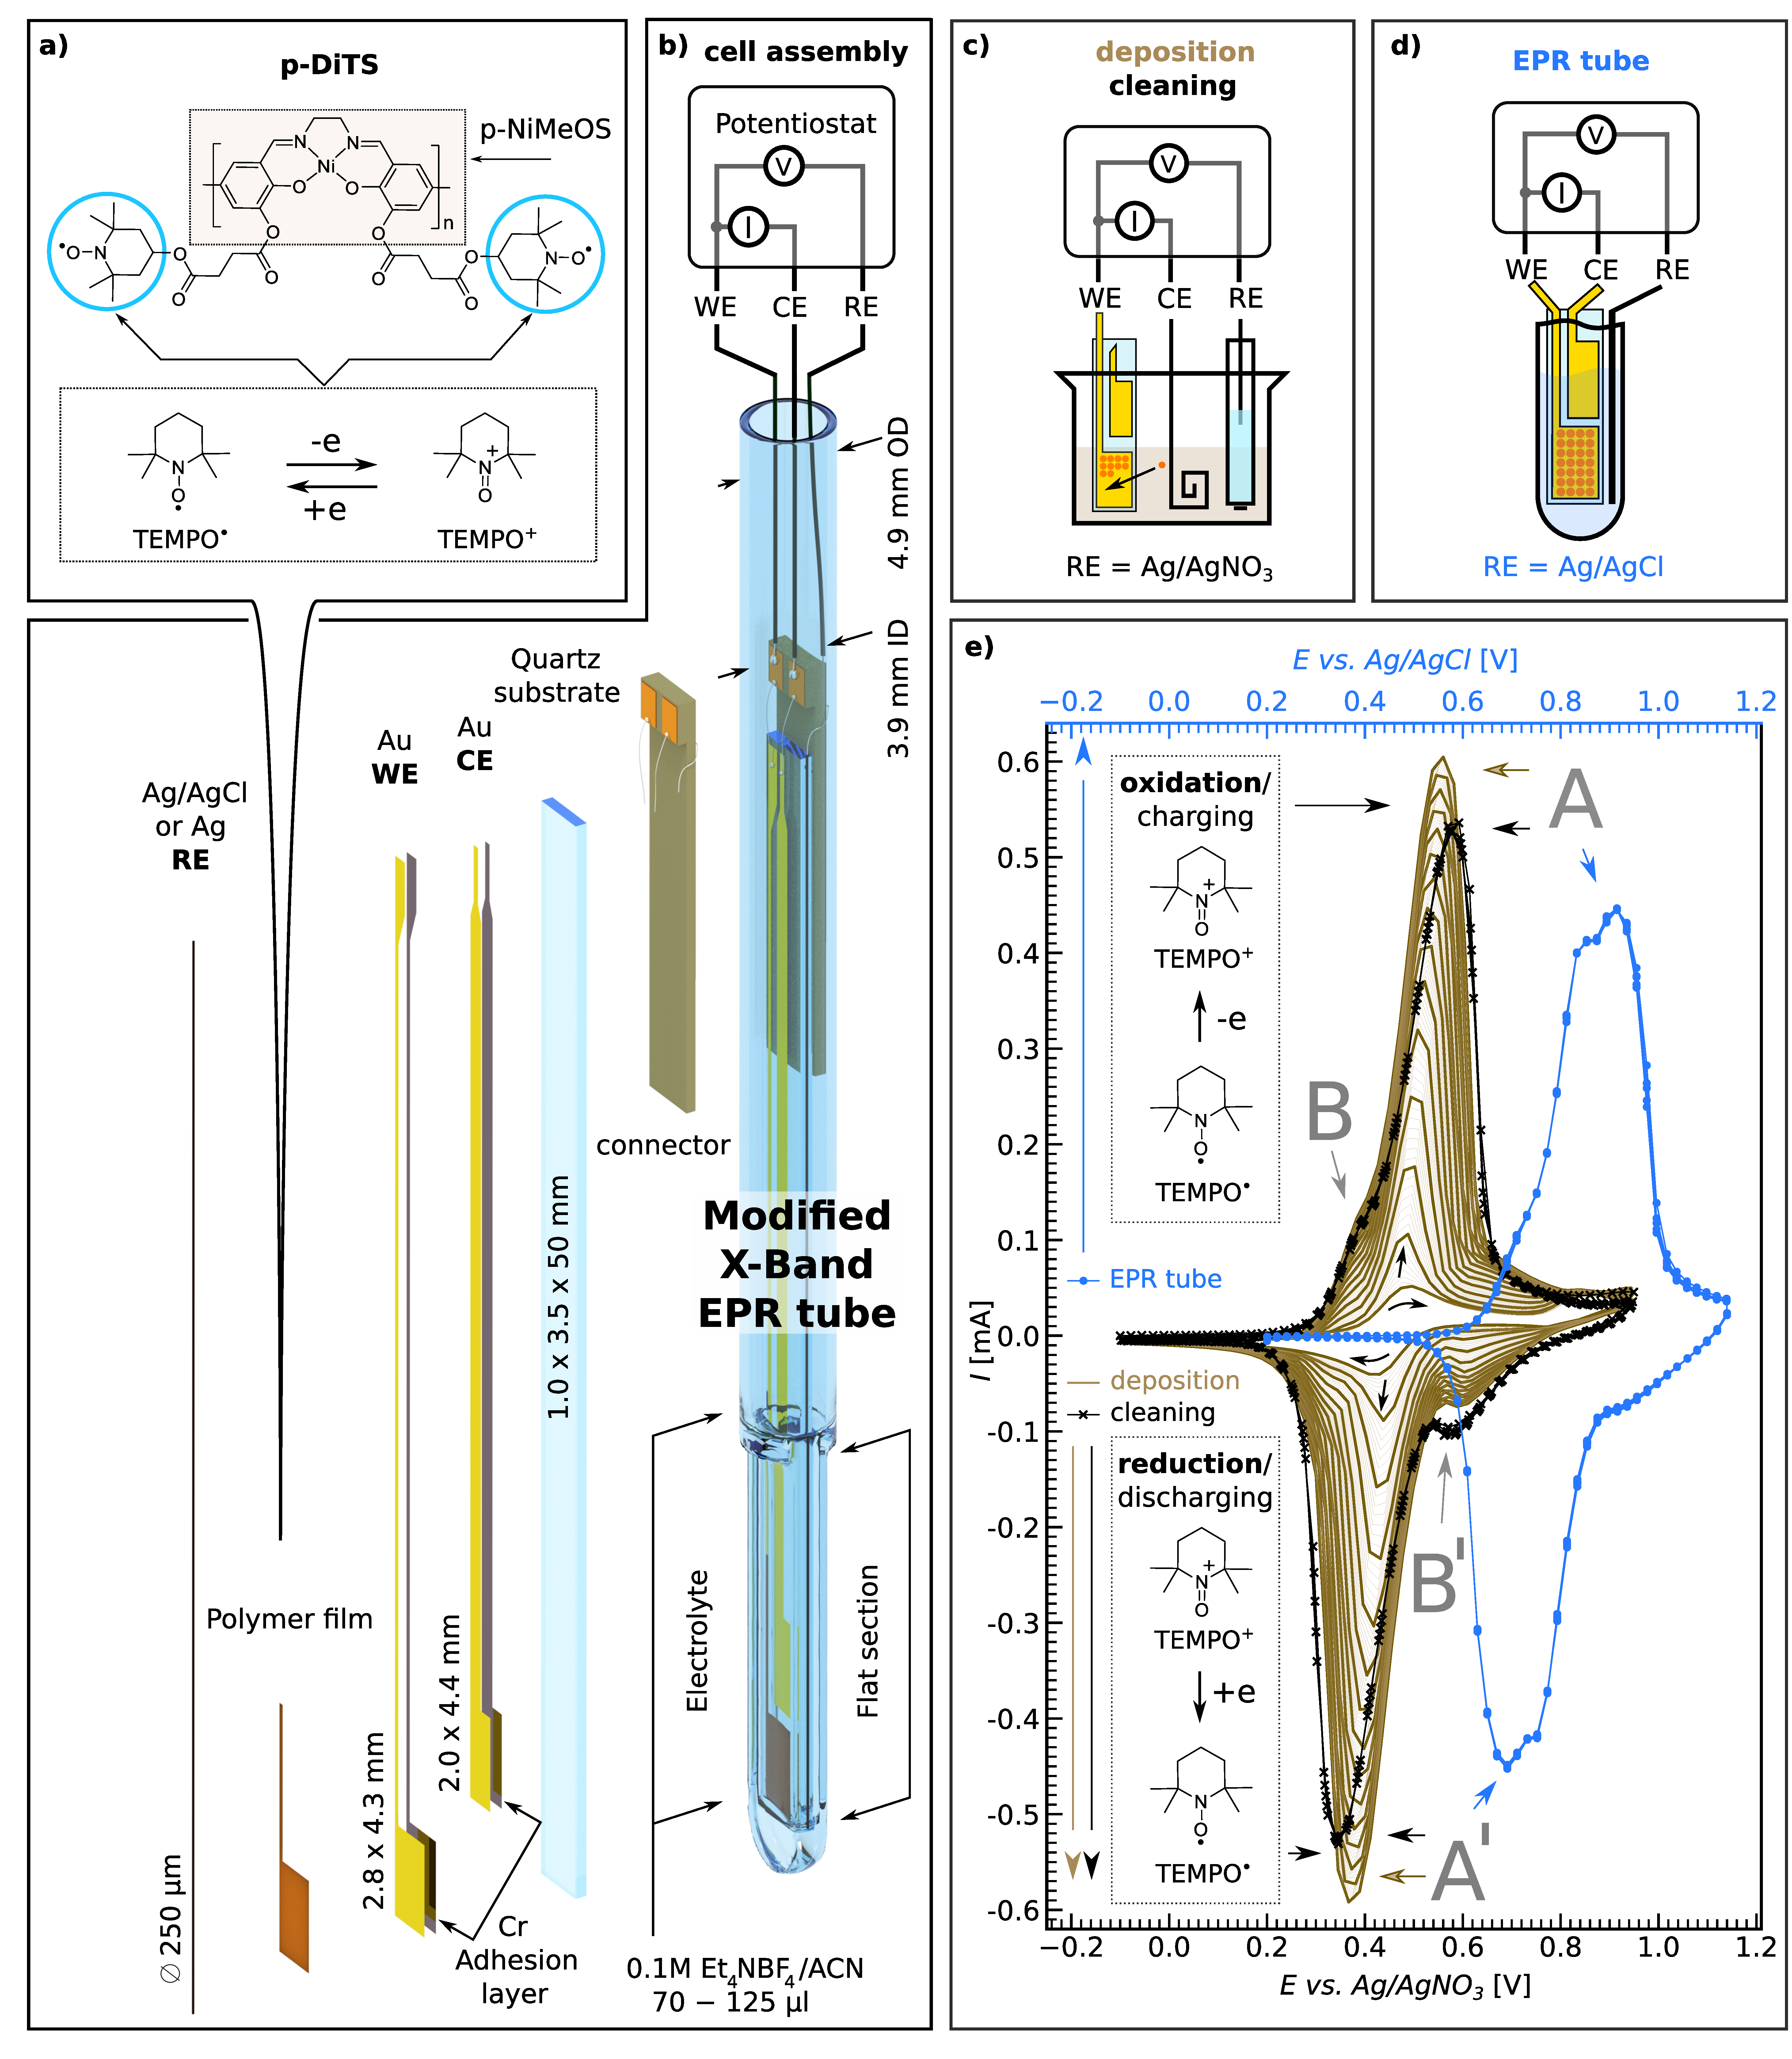
\includegraphics[width=0.99\textwidth]{./operando_epr/figures/Flat_tube_setup.pdf}
 \caption{Schematic diagram of the electrode design and assembly of the electrochemical cell based on a modified X-band EPR quartz tube. a): Molecular structure of p-DiTS, with the redox reaction of its charge-bearing TEMPO groups; highlighted is the backbone, p-NiMeOSalen. b): Photograph of the modified tube with a flattened bottom section, with the on-substrate electrochemical setup assembled inside, and the process of forming the modified tube. c): Electrochemical setup for deposition and cleaning of polymer films. d): Tube-based electrochemical setup. e): Cyclic voltammograms of a growing p-DiTS film during 100 electropolymerization cycles (solid-brown), during the cleaning process (crossed-black) and in the tube-based setup (dotted-blue). Peaks A/A', B/B' correspond to the oxidation and reduction of the TEMPO fragments and of the p-NiSalen backbone, respectively. All CV were recorded at 50~mV\,s\textsuperscript{-1}.}
 \label{fig:flat_tube}
\end{figure*}

\subsection{Versatile electrode setup for ex-situ and in-situ spectroelectrochemical EPR}
\label{electrode_setup}
%
One significant drawback with SEC EPR is the fact that microwave resonators suffer from substantial microwave damping as a result of introducing metal electrodes, polar solvents and ionic salts (i.e., the electrolyte) needed for successful electrochemistry.\cite{wadhawan2007_encofelectrochem} Microwave damping can be significantly reduced by our novel on-substrate electrode design (see Fig.~\ref{fig:flat_tube}) as this limits the amount of metal that is introduced into the resonator, while still allowing us to have electrode surface areas large enough to deposit sufficient material of interest to observe EPR signals.

\par
The on-substrate electrodes are produced as follows. Cleaned quartz substrates are placed inside a holder and covered with shadow masks. The assembly is transferred into a vacuum chamber equipped with a thermal evaporator (MBraun ProVap 5G PVD System). At a pressure of $7\times10^{-7}$~mbar, 10~nm of Chromium (Cr) adhesion layer is evaporated, followed by 180~nm of Gold (Au). In this way the on-substrate working and counter electrodes are formed (WE and CE respectively). The reference electrode (RE) is not evaporated on substrate for electrochemical stability reasons. Instead, a \SI{250}{\micro\meter} Ag wire is used, either as is or, for additional stability, coated galvanically with a AgCl layer.\cite{Safari2011} See Section \ref{Experimental_Section} in the ESI$\dag$ for details of the sample preparation.
\par
The above procedure provides a WE active area of 12.0~mm$^2$ which allows one to deposit an electrochemically active film that is large enough to yield a clear EPR signal. The flat electrode design provides the possibility to increase the WE area for samples with particularly small EPR signals while still maintaining certain film thicknesses. This also allows for studying EPR properties as a function of film thickness. In cases where the electrochemical process is thought to deposit material on both the WE and CE, the distance between the on-substrate electrodes can be adjusted such that only one of the electrodes is positioned in the active volume of the microwave resonator, allowing for selective EPR probing of either of the electrodes.
\par
The on-substrate electrodes reduce microwave damping. However, a substantial amount of microwave damping occurs due to the electrolyte, made of polar solvent and ionic salts. Therefore, we further optimize our setup by modifying conventional 5~mm outer diameter (OD) quartz EPR tubes by flattening the bottom 1.3$-$1.6~cm (cf.\ Fig.~\ref{fig:flat_tube}b and Section \ref{fig:S1_modified_tube} in the ESI$\dag$), thereby reducing the active electrolyte volume needed to submerge both the WE and CE on the substrate as well as the RE wire, from $\sim$120~$\mu^{\bullet}$L to $\sim$60$-$70~$\mu^{\bullet}$L.
\par
The flattened tube and the thin-film electrode setup have an additional benefit in that the sample is moved away from the maximum of the electric field distribution in the Bruker ER~4122-SHQE resonator (TE\textsubscript{011} mode cavity for cwEPR), thereby further increasing the resonator quality factor (Q-factor, given by $Q = \frac{\nu_{res}}{\Delta \nu}$, $\nu_{res} =$ resonance frequency, $\Delta \nu =$ FWHM of the resonance dip) and hence sensitivity. Further improvements can be made using the flat electrode setup in a TM\textsubscript{110} mode cwEPR cylindrical cavity such as a Bruker ER~4103-TM (developed for studying samples exhibiting high dielectric constants), where the flattened cell can be aligned to further reduce coupling to the microwave electric field. The modified tube is compatible with commercial Bruker ER~4118X-MD5 resonators, most commonly used for advanced pulse EPR measurements at X-band frequencies ($\nu = 9-10$~GHz).


\subsection{Fabrication of the modified tube}
%
The volume of the cell used in this study had to be minimized, as the high dielectric constant of the electrolyte does not allow for the critical coupling of the resonator. The volume of the electrolyte was minimized by flattening the tip of the quartz (melting point $T_m=1660-1710\,^{\circ}$C) tube accommodating the cell. For that, a tungsten (W, $T_m=3420\,^{\circ}$C) rod of a 3.70$\times$1.35$\,$mm rectangular cross section, narrowing to the bottom of the tube at a wedge angle of $\alpha \approx 5 ^{\circ}$, was inserted into the tube (Fig.~\ref{fig:S1_modified_tube}). The tube was evacuated and filled with He to a pressure of 100~mbar. The tip of the evacuated tube was molten around the thermally expanded rod with a Hydrogen-Oxygen burner ($T_f = 3080\,^{\circ}$C). The modified tube was then connected to atmosphere and the cooled, contracted rod was removed and later reused for modifying other tubes. The tungsten rod was fabricated from an electrode of a flash lamp of a pulsed Nd:YAG laser.\\

\begin{figure*}[h!]
\centering
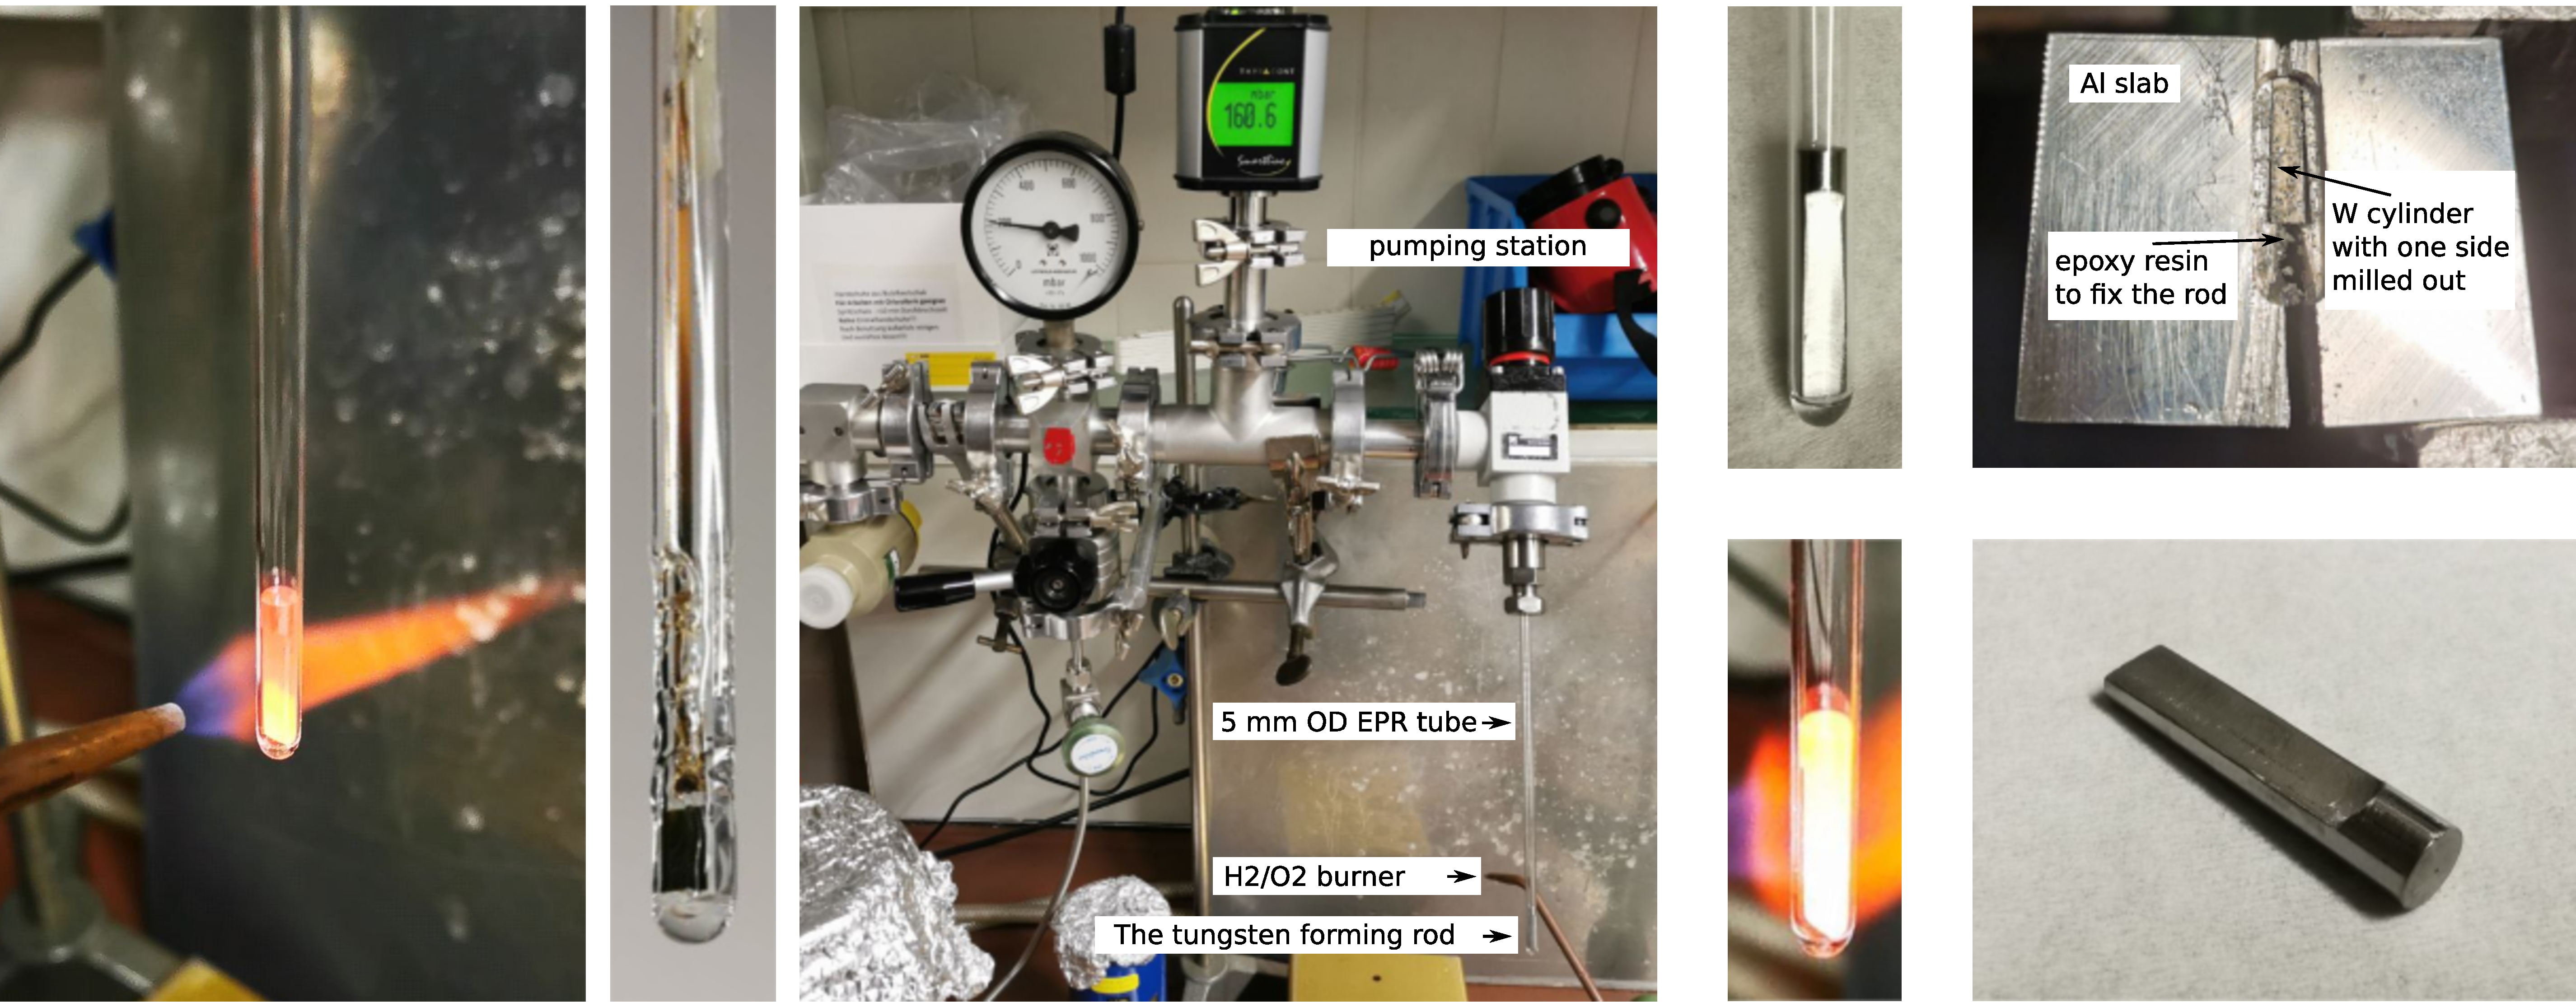
\includegraphics[width=1\textwidth]{./operando_epr/figures/spins_at_work/Figure_S1.pdf}
\caption{Modifying the tip of the standard 5~mm OD quartz EPR sample tube by melting it around a Tungsten (W) forming rod with a H$_2$/O$_2$ burner in an evacuation setup.}
\label{fig:S1_modified_tube}
\end{figure*}

The modification of the tip of the tube provided a decrease in the volume of the electrolyte down to \SI{45}{\micro\liter}, while the cylindrical part of the tube allowed for fitting the substrate connector and the wiring in. That allowed for the room temperature EPR measurements on the electrochemical cell during charging and discharging. Extensive care had to be taken to reproduce the cv curve in the modified tube as the limited volume of the electrolyte was distributed over the large surface area. That caused poor ionic transport in the electrolyte layer.\\


To establish the extent to which the modified tube improves the resonator Q-factor (Q) and therefore sensitivity of the cwEPR experiment, cwEPR spectra and associated Q-factors were recorded for a flat-electrode p-DiTS cell assembled in two different sample tubes. For both cell setups we used enough electrolyte to submerge all three electrodes. This required 100~$\mu^{\bullet}$L for the standard tube and 70~$\mu^{\bullet}$L for the modified tube. The effect of the two tubes on the cwEPR spectrum and on the Q-factor was studied for a range of heights ($H$) measured from the center of the microwave resonator to the middle of the WE.

\begin{figure}[h]

	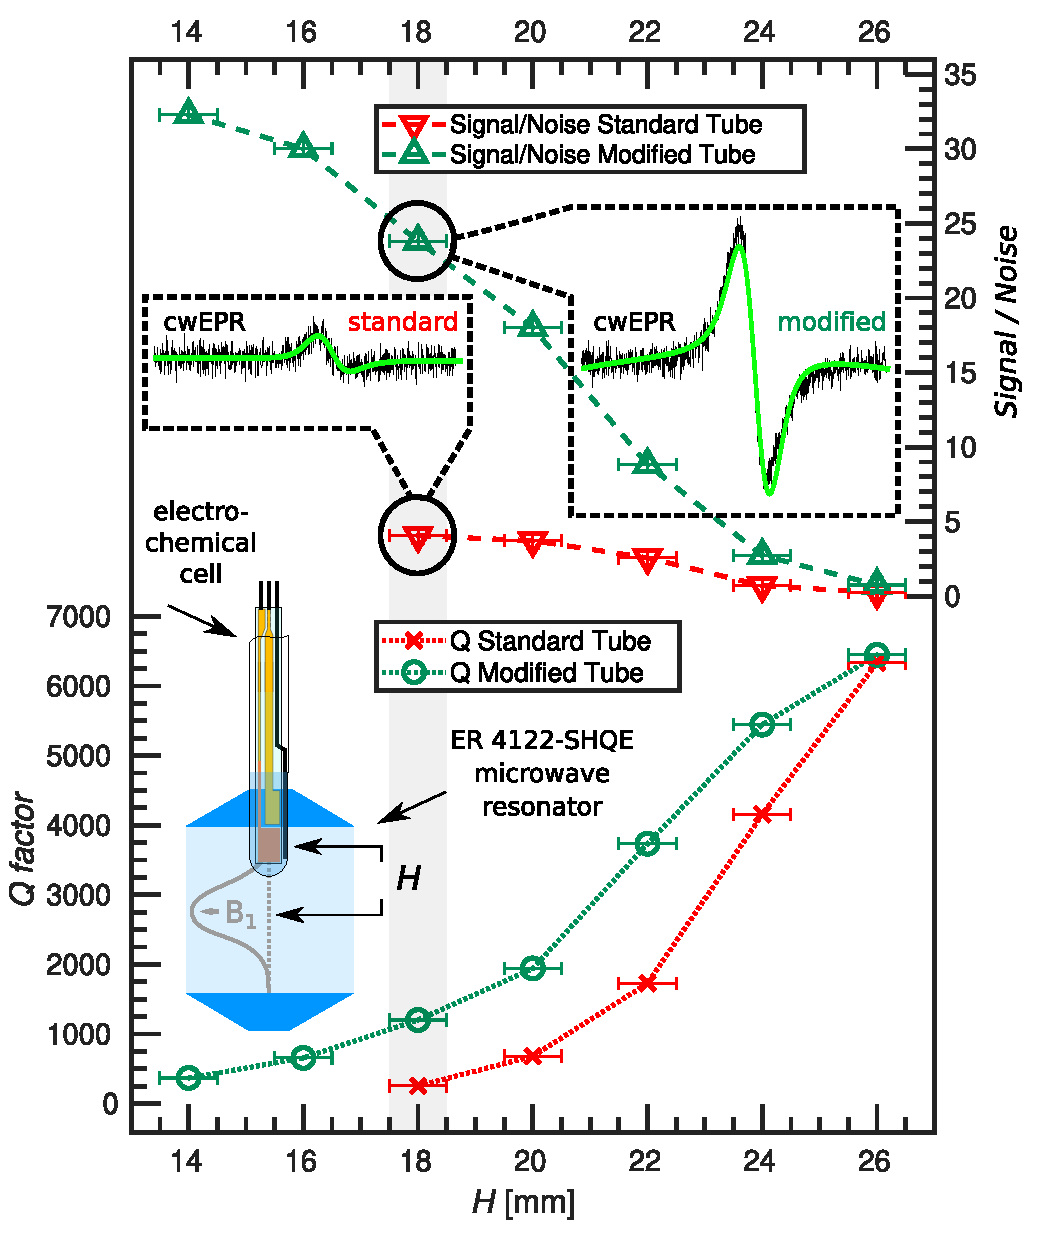
\includegraphics[width=0.5\textwidth]{./operando_epr/figures/Q_factors_mod_tube.pdf}
	\caption
	{Signal-to-noise ratio of the cwEPR spectrum of p-DiTS and the Q-factor of the Bruker ER4122-SHQE microwave resonator measured for an electrochemical cell based on a standard X-band EPR sample tube and for an electrochemical cell based on the modified tube. Data for various heights $H$ from the center of the resonator. Insets: Representative cwEPR spectra at $H=18$~mm, where the signal for the standard tube is the strongest.}
	%{Changes in the microwave resonator Q-factor when loaded with a p-DiTS sample with electrolyte in a standard and modified tube as a function of $H$.}
	\label{fig:Q_factors_mod_tube}
\end{figure}


\subsection{Q-factors and cwEPR spectra for p-DiTS in standard and modified tube}\label{Q-factor_SNR}

We determine Q~$\approx$~7800 for the empty resonator. Inserting the tube-based cells initially at $H=$~24~mm reduces the Q-factor for both cases, but more significantly for the standard tube (Q\textsubscript{standard tube}~$\approx$~4200, Q\textsubscript{modified tube}~$\approx$~5400, see Fig.~\ref{fig:Q_factors_mod_tube}). At $H=$~18~mm the Q-factor drops for both, again more significantly for the standard tube to Q\textsubscript{standard tube}~$\approx$~300 while for the modified tube it is still Q\textsubscript{modified tube}~$\approx$~1200, a factor of 4 difference. This difference between the two tubes shows the benefit of using the modified tube and flat electrode geometries for SEC EPR. When the modified tube is inserted as deep as $H=$~14~mm, the Q\textsubscript{modified tube} is around 400, which still allows for EPR measurements. Coupling the resonator not possible for $H<18$~mm (standard tube) and $H<14$~mm (modified tube).

\par
The decreasing Q-factor is not the only effect of a high-dielectric sample in an EPR resonator. The interaction between the sample and the electric field distribution of the resonator causes a mixture of absorption and dispersion signals, leading to asymmetric lineshapes in the cwEPR spectra. This makes double integration of the derivative cwEPR signal more complex, thereby making a quantitative analysis more difficult. This effect can be seen in the cwEPR spectra of p-DiTS (Fig.~\ref{fig:Q_factors_mod_tube}) measured in the standard 5~mm tube for $H=$~18~mm where the cwEPR signal is asymmetric. The modified tube yields symmetric lineshapes at the same sample heights. Further details are presented in the following subsection.

\par

The electrochemical cells based on the modified tube allow for higher EPR signals as compared to the normal X-band EPR tube. Fig.~\ref{fig:S2_Qfactor} represents two sets of measurements that describe the enhancement of the EPR signal for the modified tube. When the cell is inserted closer to the resonator's center, the Q factor of the resonator lowers and the EPR signal increases, because the intensity of the magnetic component of the microwave field B$_1$ is higher in the center of the resonator. When the cells were inserted closer to the center of the resonator, the Q factor went from $\approx$~6000 down to $\approx$~400, so that the microwave bridge could not be critically coupled to the resonator and no EPR measurements were possible. Depending on the volume of the electrolyte in the cell, it can be inserted more or less deep into the resonator.

The modified tube could be inserted 7 mm deeper into the microwave resonator (see Fig.~\ref{fig:S2_Qfactor}). The EPR signal in the modified tube is increased as compared to the normal tube at the same height.

\begin{figure*}[h]
\centering
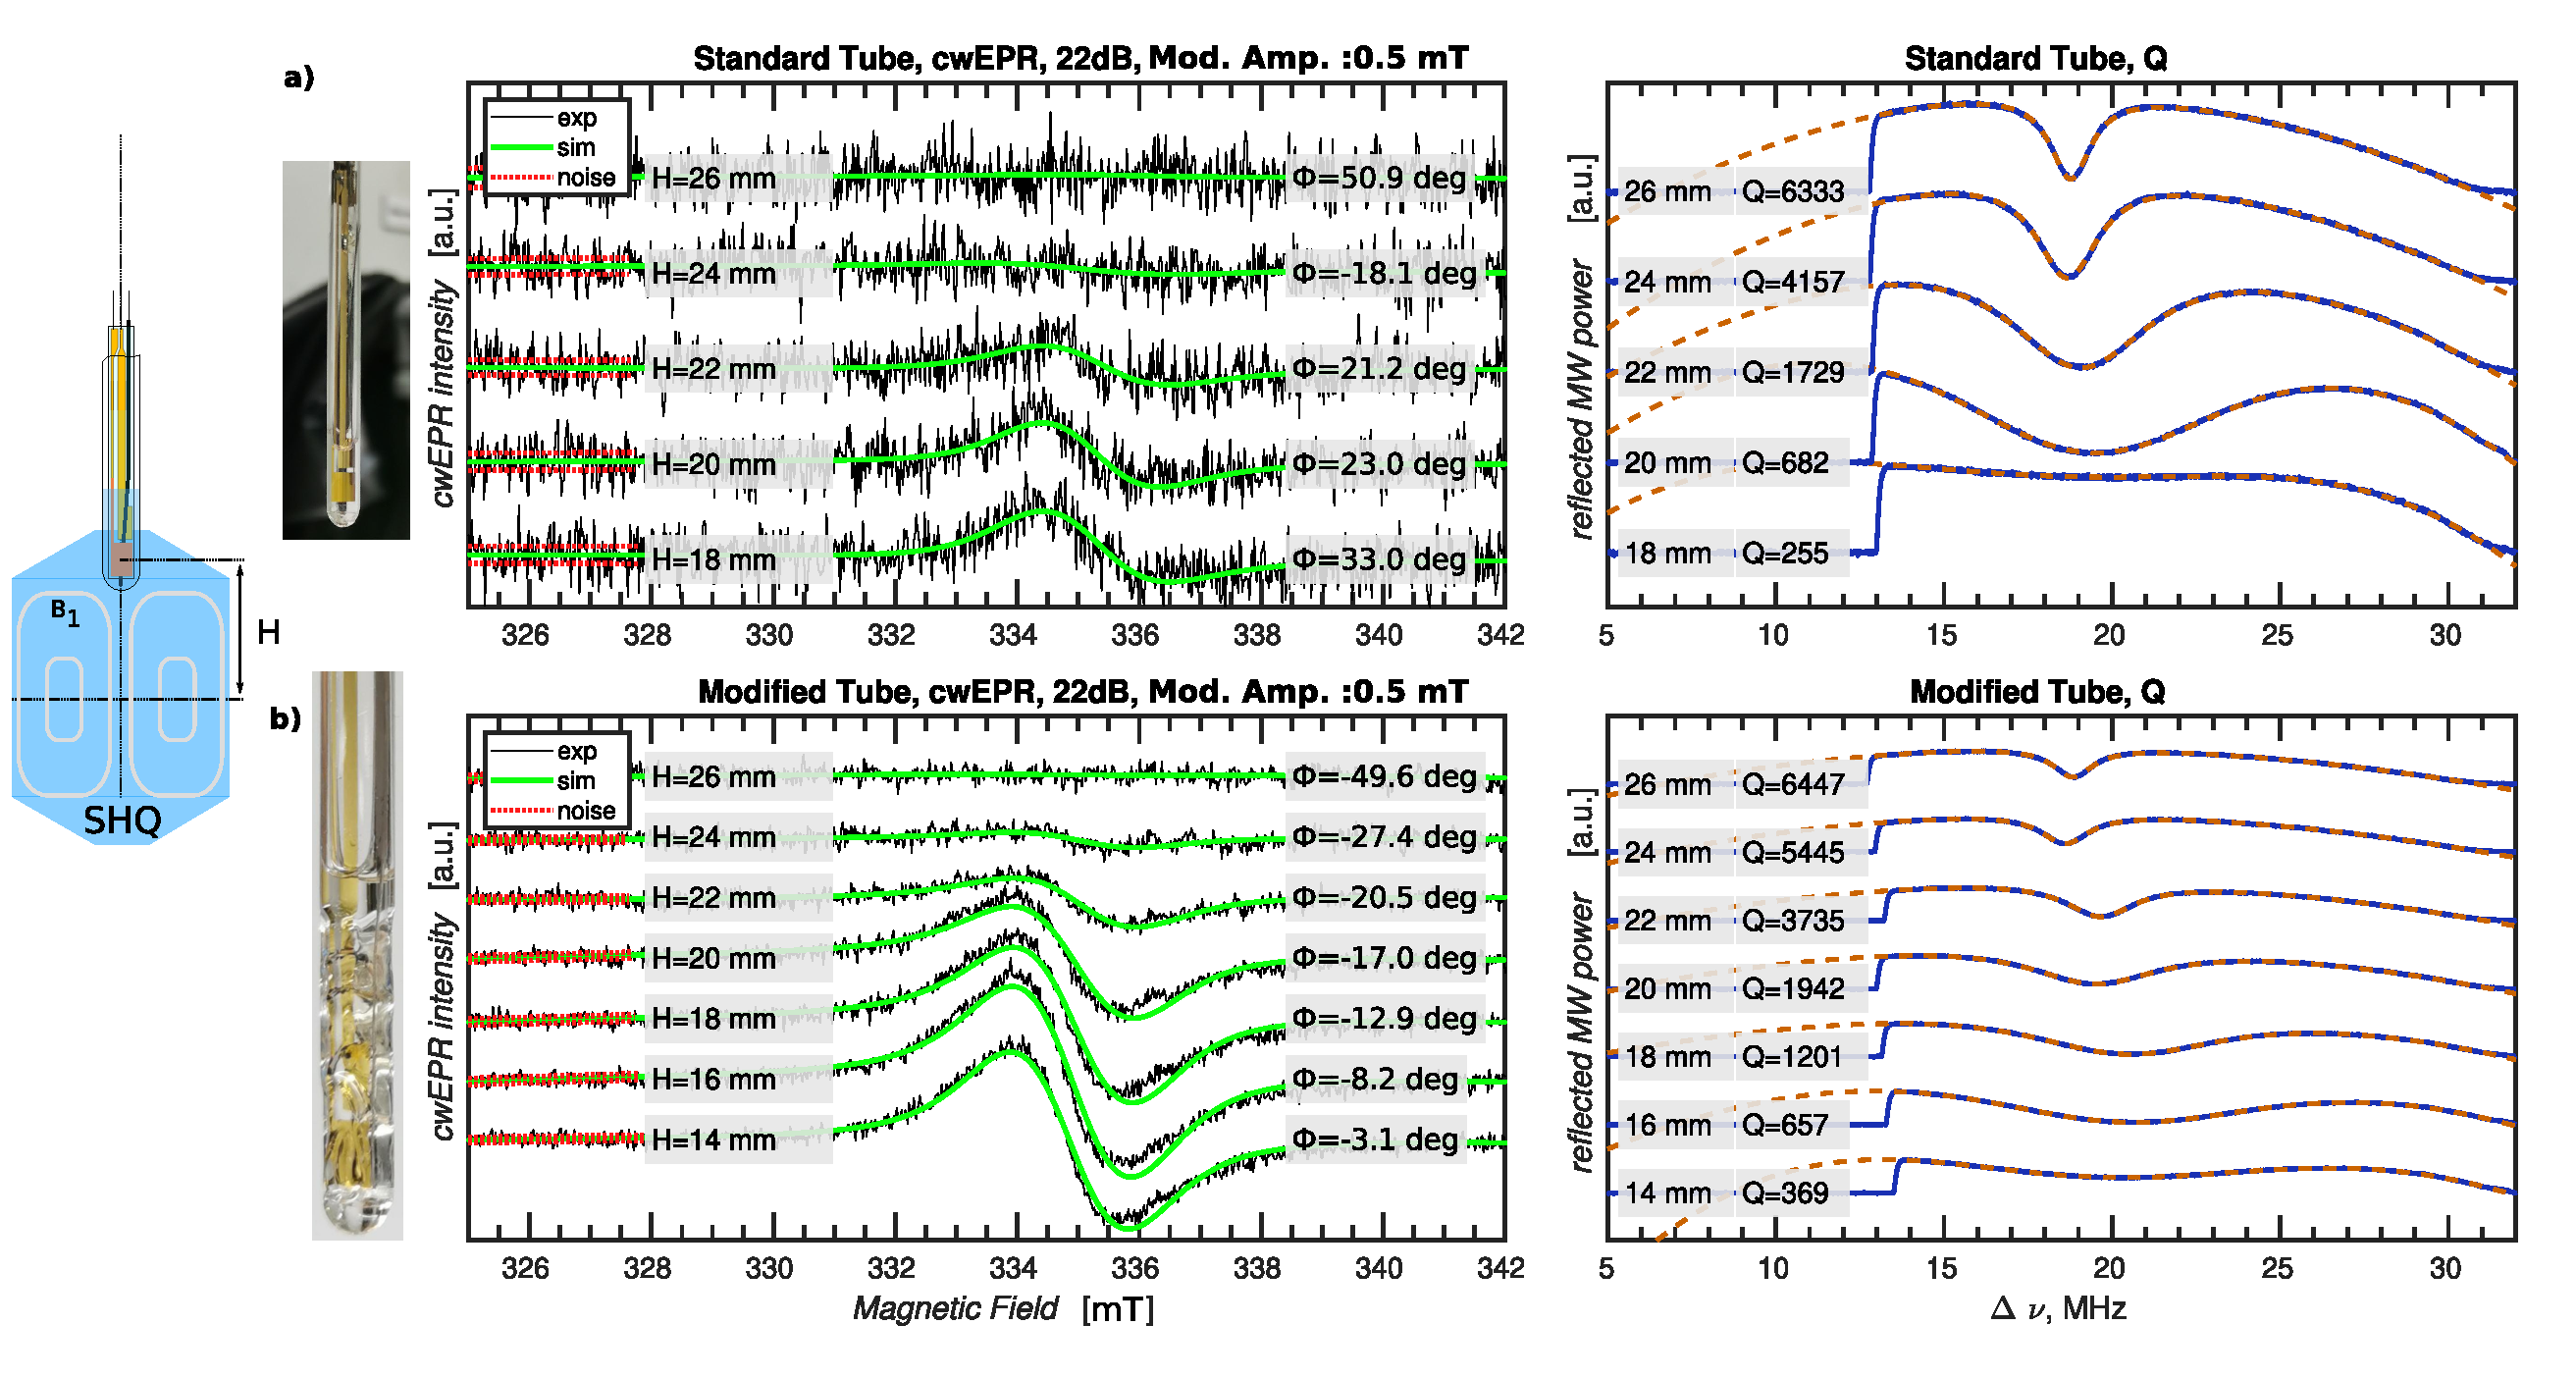
\includegraphics[width=1\textwidth]{./operando_epr/figures/spins_at_work/Figure_S2.pdf}
\caption{cwEPR signal intensity and Q factors for the standard 5~mm OD quartz EPR sample tube and for the modified tube at different heights from the center of the Bruker ER~4122-SHQE resonator. $\nu=$~9.4~GHz. Simulations of the cwEPR spectra with adjusted microwave phase. Noise analysis.}
\label{fig:S2_Qfactor}
\end{figure*}

\par
The modified tube also allows for larger cwEPR signal intensities as it can be inserted closer to the resonator center. The signal-to-noise ratio (S/N) for the modified tube is increased by a factor of $\approx$6 as compared to the standard tube, both inserted at $H=$18~mm. At the maximum sample insertion, the S/N is improved by a factor of $\approx$8 for the modified tube.
\par
Using the modified tube we see three major benefits. Firstly, it results in much higher Q-factors and therefore sensitivity when comparing Q-factors for the same sample height. Secondly, the modified tube allows for insertion of the tube closer to the resonator center, allowing for a larger S/N and therefore requiring less averaging time for each cwEPR measurement. This is especially useful for samples where holding the potential for long periods causes unwanted effects or degradation. Thirdly, cwEPR measurements with the modified tube give symmetric cwEPR lineshapes (using the conventional procedure for critically coupling the microwave cavity, the standard tube gives an asymmetric lineshape) which allows for more straightforward quantitative analysis (spin counting), especially useful for in-situ cwEPR with varying redox potentials.





\section{cwEPR Spectroscopy of a Charging Electrochemical Cell}
There is a number of difficulties when it comes to an EPR experiment on a working electrochemical cell. The cell must contain mobile ions between its electrodes - cations and anions. The ions are normally produced as products of dissociating salts. To overcome the ionic bond in a salt and to break it into the ions, a solvent with large dipole moment is needed. Solvents with large dipole moments, as acetonitrile (CH\textsubscript{3}CN, $\epsilon\approx 37.5$) or water ($\epsilon\approx78.4$), have large dielectric constants which results in a non-resonant absorption of microwaves. A cell containing liquid electrolyte absorbs microwaves and lowers the sensitivity of the EPR experiment. Furthermore, due to a finite dimension of cell, not only the magnetic component of the microwave is interacting with the electrolyte, but also the electric one - this results in heating of the electrolyte in a similar fashion as in a microwave oven. The heating of the electrolyte leads to a faster degradation of the cell and does not allow for long systematic measurements.\\
Another general issue with the operando EPR and EDMR experiments is that the device under testing (DUT) has to have metal electrodes that deliver current to it. Metals, placed in a microwave cavity, change the distribution of the electromagnetic field in it - that weakens the magnetic component at the device and at the same time strengthens the electric component. It is the magnetic dipole transition that is causing the magnetic resonance, so the weakening of the magnetic component by introducing the metal electrodes further decreases the magnetic resonance response. The increased electric component causes heating to temperatures that can be critical for the DUT operation.



\subsection{cwEPR Spectra During a Charge-Discharge Cycle}
There are four characteristic cwEPR signatures of an electrochemical cell containing di-TEMPO-Salen polymer cathode. The well known signature of a freely tumbling TEMPO$^{\bullet}$ exhibits three narrow lines corresponding to the three nuclear sublevels of nitrogen: $m_I=-1,0,+1$.
\begin{figure}[h]
\center
	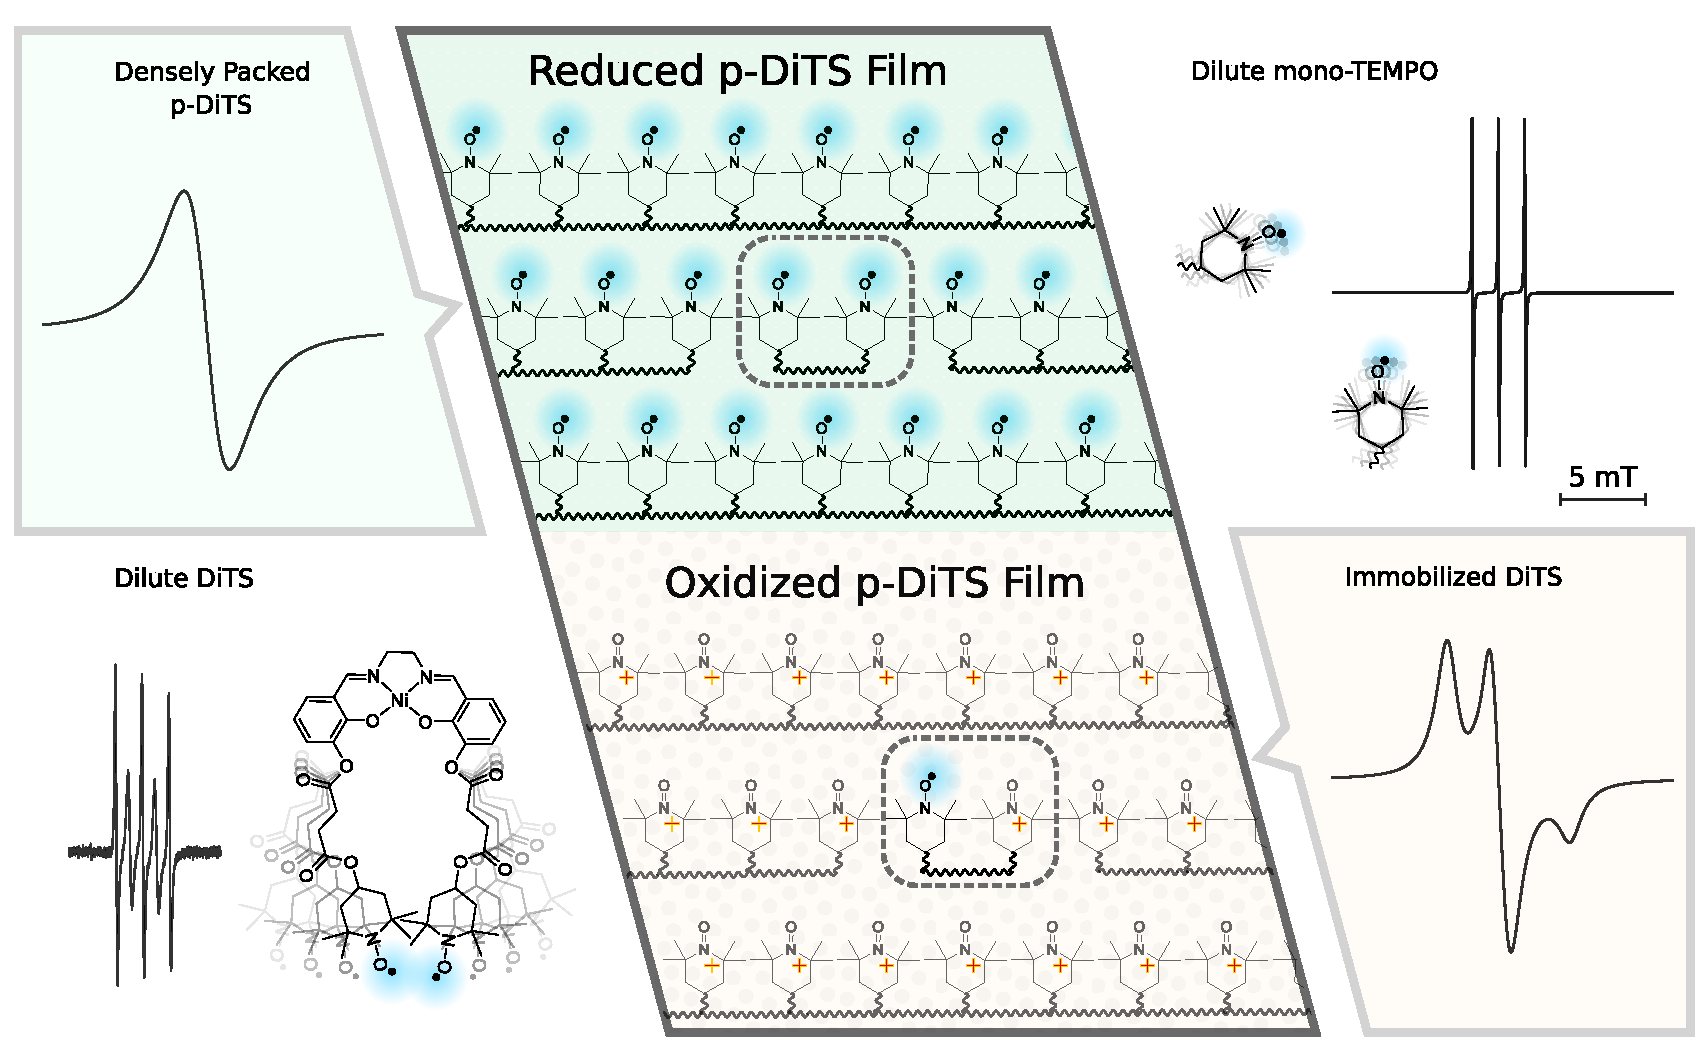
\includegraphics[width=1\textwidth]{./operando_epr/figures/Cartoon_ALL.pdf}
	\caption{Classification of the nitroxide cwEPR spectra observed for p-DiTS under different conditions and in different environments. a): Densely packed nitroxide film with dipolar broadening and exchange narrowing or broadening giving a single derivative line. b): Typical spectrum of dilute mono-nitroxide in solution, three-lines due to $S=1/2$, $I=1$ $^{14}$N hyperfine interaction (described by isotropic $g$-factor and isotropic hyperfine ($A$) interaction). c): Typical spectrum of tumbling di-nitroxide in solution where dynamic changes in the nitroxide -- nitroxide distance modulate the exchange interaction yielding a five-line structure with alternating line width (measured cwEPR of DiTS monomers in solution at room temperature). d): Immobilized nitroxide spectrum with both $g$ and $A$ anisotropy.}
	\label{fig:cartoon_spectra_dts}
\end{figure}


EPR spectra of electrochemical cells with p-DiTS as active-electrode material can exhibit a variety of different signals. Before presenting and discussing the experimental results, we will provide an overview about the various characteristic cwEPR lineshapes associated with nitroxides in different environments.
\par

Fig.~\ref{fig:cartoon_spectra_dts}a shows the spectrum expected for a \emph{densely packed p-DiTS film} with all nitroxides in the EPR-active reduced state. The broad unstructured line results from the strong dipolar and exchange interaction between both nitroxides of each DiTS monomer as well as between the nitroxides of different monomers. The exchange interaction can lead to either line narrowing or broadening depending on the strength of the interaction,\cite{Anderson1953} while the dipolar interaction causes broadening. In consequence, the overall cwEPR line width depends on the spin concentration in the film.
\par 
\emph{Dilute mono-TEMPO fragments} dissolved in the electrolyte, each containing only one nitroxide, give rise to a three-line spectrum (cf.\ Fig.~\ref{fig:cartoon_spectra_dts}b) which is well known from nitroxide-based spin labels in solution.\cite{Liu_2008} Tumbling of the molecules in the liquid electrolyte results in an averaging of the anisotropic interaction between the electron spin and the nitrogen nuclear spin ($I = 1$) as well as of the $g$ anisotropy, leaving only the isotropic part of the hyperfine coupling and the isotropic $g$ value. 
\par
\emph{Dilute DiTS monomers} in the electrolyte generally give a spectrum consisting of five narrow lines (cf.\ Fig.~\ref{fig:cartoon_spectra_dts}c), if each monomer contains two interacting EPR-active nitroxides. The spectrum depends on dynamic effects, specifically the modulation of the exchange interaction between both radicals of each monomer.  Thus, depending on the solvent and temperature, the spectrum can be indistinguishable from the three-line spectrum of mono-TEMPO fragments.
\par
The fully charged (oxidized) p-DiTS film can contain electrically isolated domains in which the nitroxides are not connected to the electrode and cannot be oxidized or reduced. These electrically inactive \emph{immobilized DiTS monomers} in the oxidized film display a spectrum as shown in Fig.~\ref{fig:cartoon_spectra_dts}d. In contrast to the densely packed p-DiTS film, the dipolar and exchange interactions between neighboring radicals are much weaker. The anisotropy of the nitroxide's hyperfine tensor adds features to the cwEPR spectrum in d) as compared to a).
Yet, there is some remaining line broadening that does not allow one to distinguish between immobilized DiTS monomers with either one or two paramagnetic nitroxides.
\par
We note that the oxidized NiSalen backbone can contribute to the spectrum as well. Its EPR signature, which is not shown in Fig.~\ref{fig:cartoon_spectra_dts}, is clearly different from the nitroxide/TEMPO-related spectra discussed above.
%


\subsection{Spectral Simulations}

\subsection{Quantitative Analysis of Potential-Dependent EPR Spectra}
\label{sec:quantitative_EPR}
\begin{figure}[!ht]
\center
	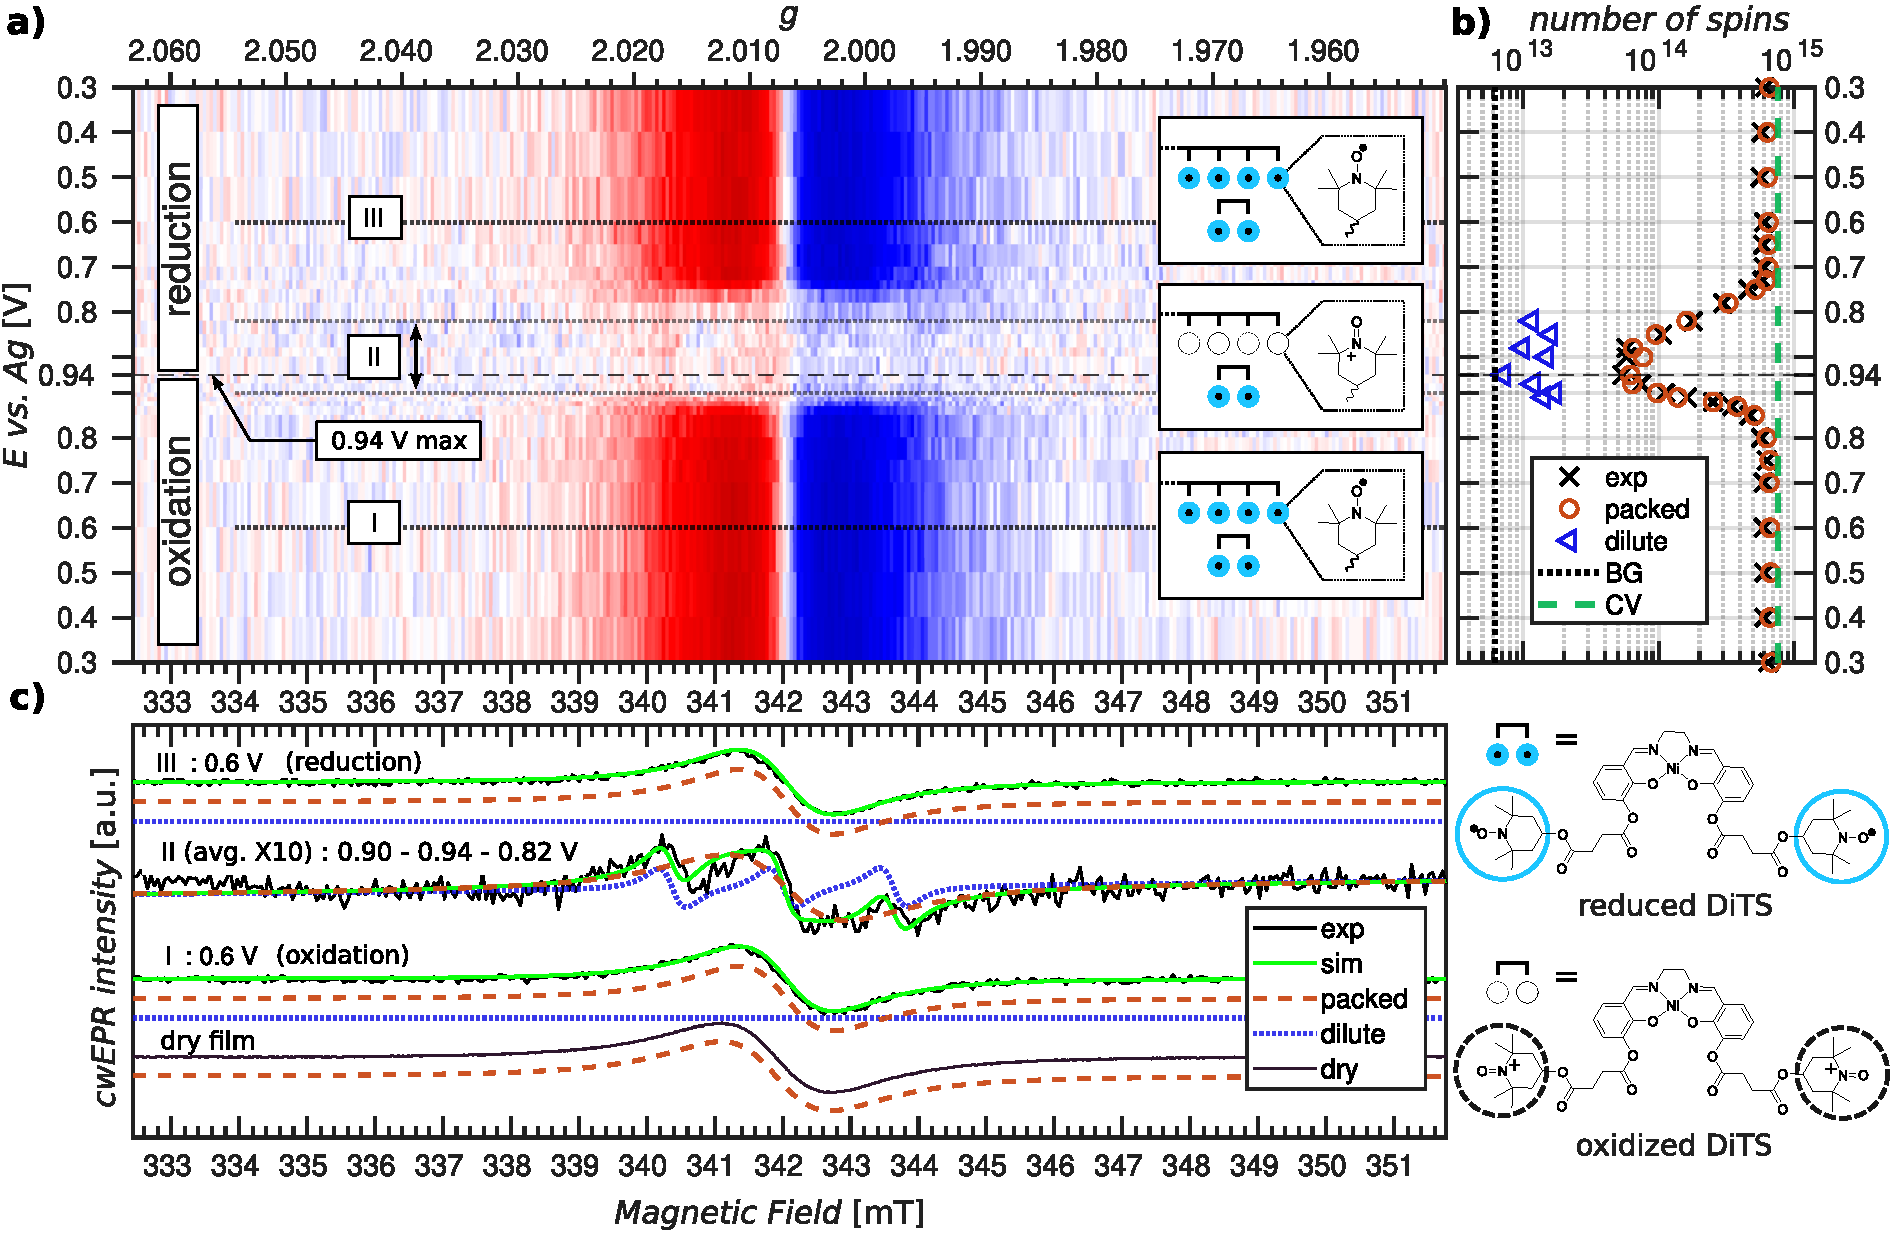
\includegraphics[width=1\textwidth]{./operando_epr/figures/Main_2D_redox_map_full.pdf}
	\caption{XXX}
	\label{fig:operando_carpet}
\end{figure}
The number of spins at each SoC was determined with quantitative cwEPR from the double integral of the cwEPR intensity calculated with the Spincounting Toolbox~\cite{spin_counting_tb} for Matlab~\cite{SI:Matlab}. The cwEPR spectra in Figure~\ref{fig:Figure_S6} were measured in a Bruker Elexsys E580 spectrometer equipped with an ER 4118 X-MD5 dielectric ring resonator with an unknown Q factor. To calibrate the intensity of the measured cwEPR signals and to determine the absolute number of spins in the film, we measured the cwEPR spectrum of the fully discharged film (SoC 0\%) with a calibrated spectrometer. The calibrated spectrometer is a lab-built X-band cwEPR spectrometer equipped with a 9.4~GHz, 200~mW microwave source and a 4122-SHQE resonator. With Q~$=6095$, the absolute number of spins in the pDiTBuS film at SoC~0\% was measured to be $N=(6.9\pm0.4)\times10^{15}$. We used $N$ to get the number of spins for other SoC from the spectra measured with the uncalibrated spectrometer. We assumed that the Q factor of the resonator remains the same for different SoC~\cite{Kulikov2022_SI} and computed the corresponding numbers of spins from the doubly integrated spectral intensities.\\

The doubly integrated cwEPR spectral intensities for the pDiTBuS film in the four considered SoC relate to each other as 100:51:15:6 with the absolute number of spins of $(6.9\pm0.4)\times10^{15}$, $(3.5\pm0.2)\times10^{15}$, $(1.1\pm0.1)\times10^{15}$ and $(3.8\pm0.4)\times10^{14}$, respectively. The respective ESOC are therefore $(0\pm5)$\%, $(49\pm3)$\%, $(85\pm2)$\% and $(95\pm1)$\%. Spin \rs{concentrations} in the film are $(5.3\pm2.7)\times10^{20}$, $(2.7\pm1.4)\times10^{20}$, $(0.8\pm0.4)\times10^{20}$ and $(0.3\pm0.2)\times10^{20}$ cm$^{-3}$, respectively. Integration of the cyclic voltammogram yields $(2.3\pm0.8)\times10^{16}$ electrons in the reduced state.\\
%The relative intensities of the CWEPR signals correspond to ESOC 0\%, 49\%, 85\% and 95\%.
%\newpage
\begin{figure}[h]
\center
	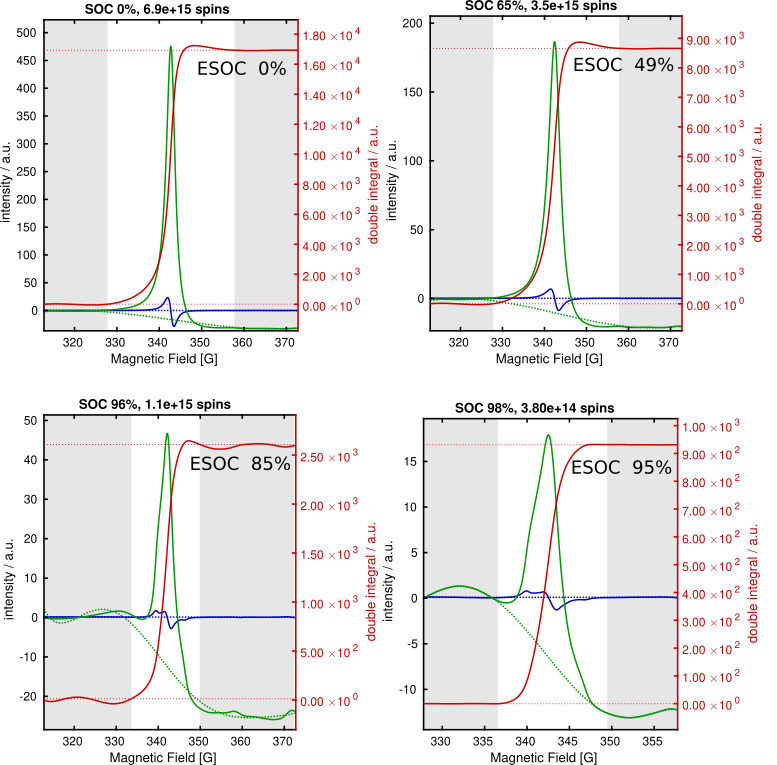
\includegraphics[width=0.85\textwidth]{./pulse/figures/Figure_S6}
	\caption{cwEPR spectra for a pDiTBuS film in four charge states. Single and double integrals of the signal. Spin count is proportional to the end value of the double integral. Temperature: 80~K, $\nu\approx$~9.6~GHz, field modulation: 5~G at 100~kHz. ER~4118 X-MD5 dielectric ring resonator.}
	\label{fig:Figure_S6}
\end{figure}




\section{EPR-Detected State Of Charge}
\label{sec:ESOC}

The SoC of the film determined with Coulomb counting were compared to quantitative cwEPR to directly relate the \ik{number of charges, injected into the film upon charging}\rs{,} to the number of paramagnetic centres in it. We refer to the \ik{fraction} of spins removed from the \ik{fully discharged} film \ik{to reach} a given SoC as the EPR-detected state of charge, or ESOC. The fully discharged film has the maximum number of spins and its ESOC is 0\%. ESOC at other SoC are determined as the fraction of the missing spins with respect to ESOC 0\%. ESOC of 95\% \rs{thus} corresponds to the oxidation state where only 5\% of the \ik{initially present} spins are left in the film. The cwEPR spectra were recorded for the listed SoC\rs{,} and the corresponding numbers of spins were calculated from the double integrals of the spectra. The integrated spectra and the experimental details are shown in the ESI, Section~\ref{si:ESOC}. \ik{The injected charges, detected spins and} ESOC values are counted for each SoC in Table~\ref{tab:Table1}. The average spin concentration in the film \rs{$\langle n\rangle$} at each ESOC was calculated from the corresponding number of spins and the estimated volume of the film of $\left(1.3\pm0.6\right)\times10^{-5}$cm$^{3}$.


\begin{table*}[!ht]

	\begin{adjustbox}{max width=\textwidth}
	 
    \begin{tblr}{ |r|c|c|c|c|c|c|c|c|}
        \toprule
E [mV] & 
SoC & 
ESOC &
capacity drawn [$\muup$Ah]& 
\ik{charges injected}&
spins \ik{detected}&
$n_{C}$~[cm$^{-3}$]&
$\langle n \rangle$~[cm$^{-3}$]&
$C$~[cm$^{-3}$] \\
		
\midrule

$ 590 \pm 5$&
$98\%$&
$(95\pm1)\%$&
\ik{$0.020\pm0.005$}&
\q{$(5\pm1)\times10^{14}$}&
\q{$(4\pm1)\times10^{14}$}&
\q{$(3\pm2)\times10^{19}$}&
\q{$(3\pm2)\times10^{19}$}&
\q{$>1\times10^{19}$}\\

\addlinespace[-0.5ex]
    
$ 500 \pm 5$&
$96\%$&
$(85\pm2)\%$&
\ik{$0.060\pm0.005$}&
\ik{$(1.4\pm0.1)\times10^{15}$}&
$(1.1\pm0.1)\times10^{15}$&
\ik{$(1.0\pm0.5)\times10^{20}$}&
\q{$(8\pm4)\times10^{19}$}&
\q{$>3\times10^{19}$}\\

\addlinespace[-0.5ex]

$ 430 \pm 5$&
$65\%$&
$(49\pm3)\%$& 
\ik{$0.480\pm0.005$}&
\ik{$(1.07\pm0.01)\times10^{16}$}&
$(3.5\pm0.2)\times10^{15}$&
\q{$(8\pm4)\times10^{20}$}&
\q{$(3\pm2)\times10^{20}$}&
$-$\\

\addlinespace[-0.5ex]

$ -200\pm 5$&
$0\%$&
$(0\pm5)\%$& 
\ik{$1.360\pm0.005$}&
\ik{$(3.05\pm0.01)\times10^{16}$}&
$(6.9\pm0.4)\times10^{15}$&
\q{$(2\pm1)\times10^{21}$}& %0.0346    0.1037    0.8297    2.3509
\q{$(5\pm3)\times10^{20}$}&
$-$\\    

        \bottomrule
    \end{tblr}
	\end{adjustbox}
	
	
\caption{EPR-detected state of charge, \ik{Coulomb counting} and the corresponding spin concentrations in a \ik{galvanostatically discharging} pDiTBuS film \ik{with $I=-10~\muup A$}. The electric potential of the film $E$ was measured with respect to the Ag/AgNO$_3$ RE. \ik{The number of injected (negative) elementary charges \rs{and the corresponding concentration of charges $n_C$ were} determined from the drawn capacity}. The average spin concentration $\langle n \rangle$ is the ratio between the number of spins measured with quantitative cwEPR and the volume of the film determined by integrating the cyclic voltammogram. $C$ is the local spin concentration in the film \ik{estimated} with \q{p}EPR as described in text.}
	
	\label{tab:Table1}	
	
	
\end{table*}

\subsection{Formation of Singlet Spin States in a Reduced Cathode Film}
The number of electrons left in the film were determined with the Coulomb counting from the galvanostatic discharge curves shown in Figure~\ref{fig:Figure_S27}. The number of electron spins detected with cwEPR is close to the Coulomb counting for high SoC, that corresponds to lower spin concentrations. However, for low SoC, the difference in the number of electrons measured with the Coulomb counting and with quantitative cwEPR is dramatic: up to 70\% of the electrons in the discharged film are EPR silent. The absence of cwEPR signal from the majority of the electrons indicates that their spins pair up in singlet (S=0) EPR silent states. The singlet spin pairs follow Bose statistics and can occupy the same quantum state which is favorable for the charge transport. The formation of singlet states was detected only in low SoC.

\section{Monitoring of Degradation Processes}
The operando monitoring of EPR spectra in pDiTS cells has revealed that the amount of paramagnetic species reduces upon the cycling. The cwEPR spectra during one charge-discharge cycle of two different pDiTS cells are shown in Figure~\ref{fig:operando_degradation}. Both datasets show a significant amount of the three-line structure in the oxidised (fully charged) state, that corresponds to the the release of dilute nitroxide radicals from the polymer film to the electrolyte. The fact that the released species exhibit a 3-line structure and not a 5-line structure excludes the release of the di-TEMPO (DiTS) monomers and suggests that individual TEMPO$^{\bullet}$ fragments are being detached from the film. Therefore, it was found that it is the molecular degradation of DiTS that is responsible for the loss of cell's capacity and not the decomposition of the polymer film into the monomer fragments. The overall EPR signal intensity decreases for both samples after the charge-discharge cycle. The spectral deconvolution with quantitative analysis of the individual components has revealed that the released fragments do not explain the overall loss of the signal intensity after the cycle.


\begin{figure}[!h]
\center
	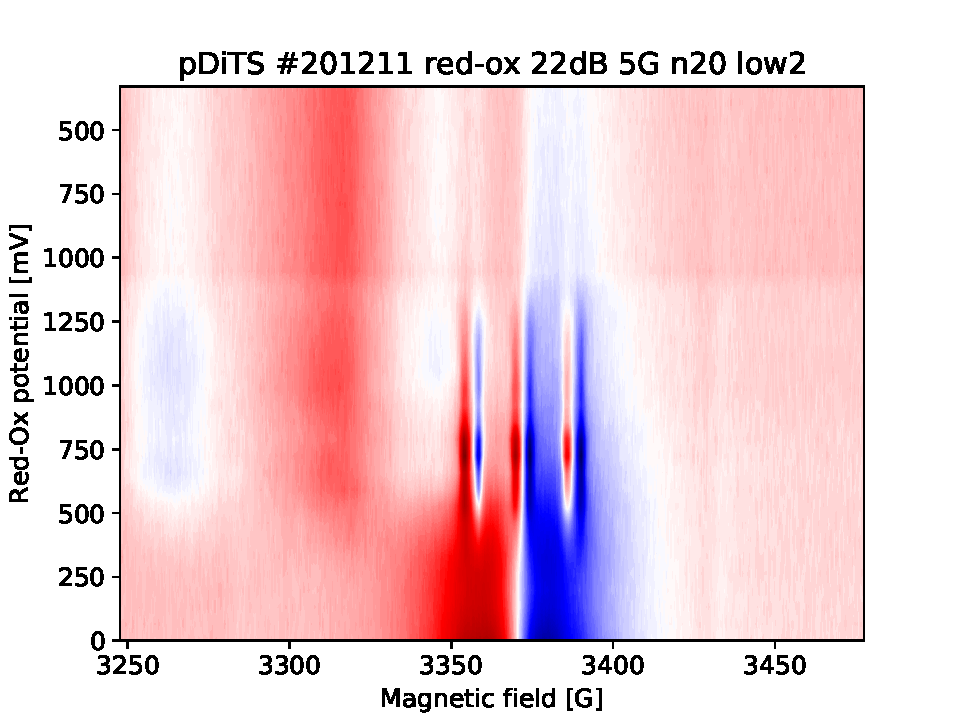
\includegraphics[width=1\textwidth]{./operando_epr/figures/degradation/overnight_dits_201211_full_redox_contour_XY.pdf}
	\caption{Operando cwEPR spectra of a pDiTS electrochemical cell showing irreversible release of charge-bearing fragments and decomposition of the device upon potentiostatic charging with currents up to $I<0.2$~mA~$\approx125$~C.}
	\label{fig:operando_degradation_device}
\end{figure}


\begin{figure}[!h]
\center
	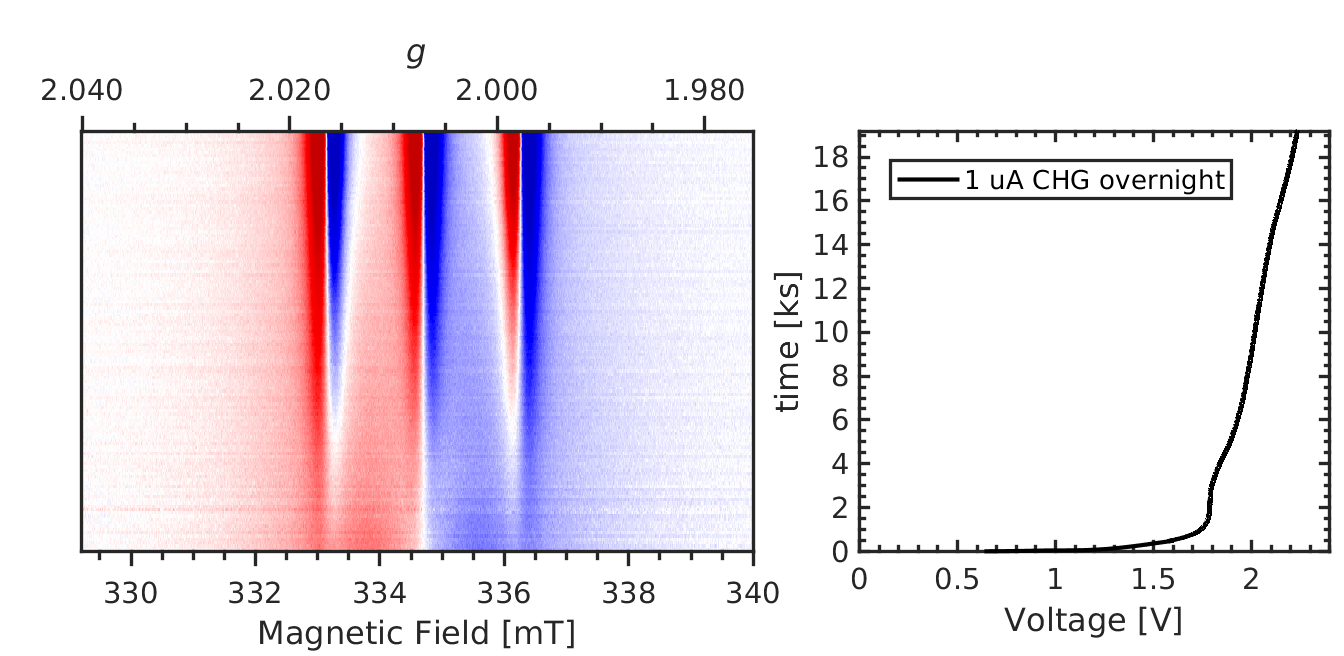
\includegraphics[width=1\textwidth]{./operando_epr/figures/degradation/pDiTS_slow_charge_MS5000_forslides.png}
	\caption{Operando cwEPR spectra of a pDiTS electrochemical cell showing irreversible release of charge-bearing fragments upon moderate charging currents.}
	\label{fig:operando_degradation_3_lines_release}
\end{figure}


\begin{figure}[!h]
\center
	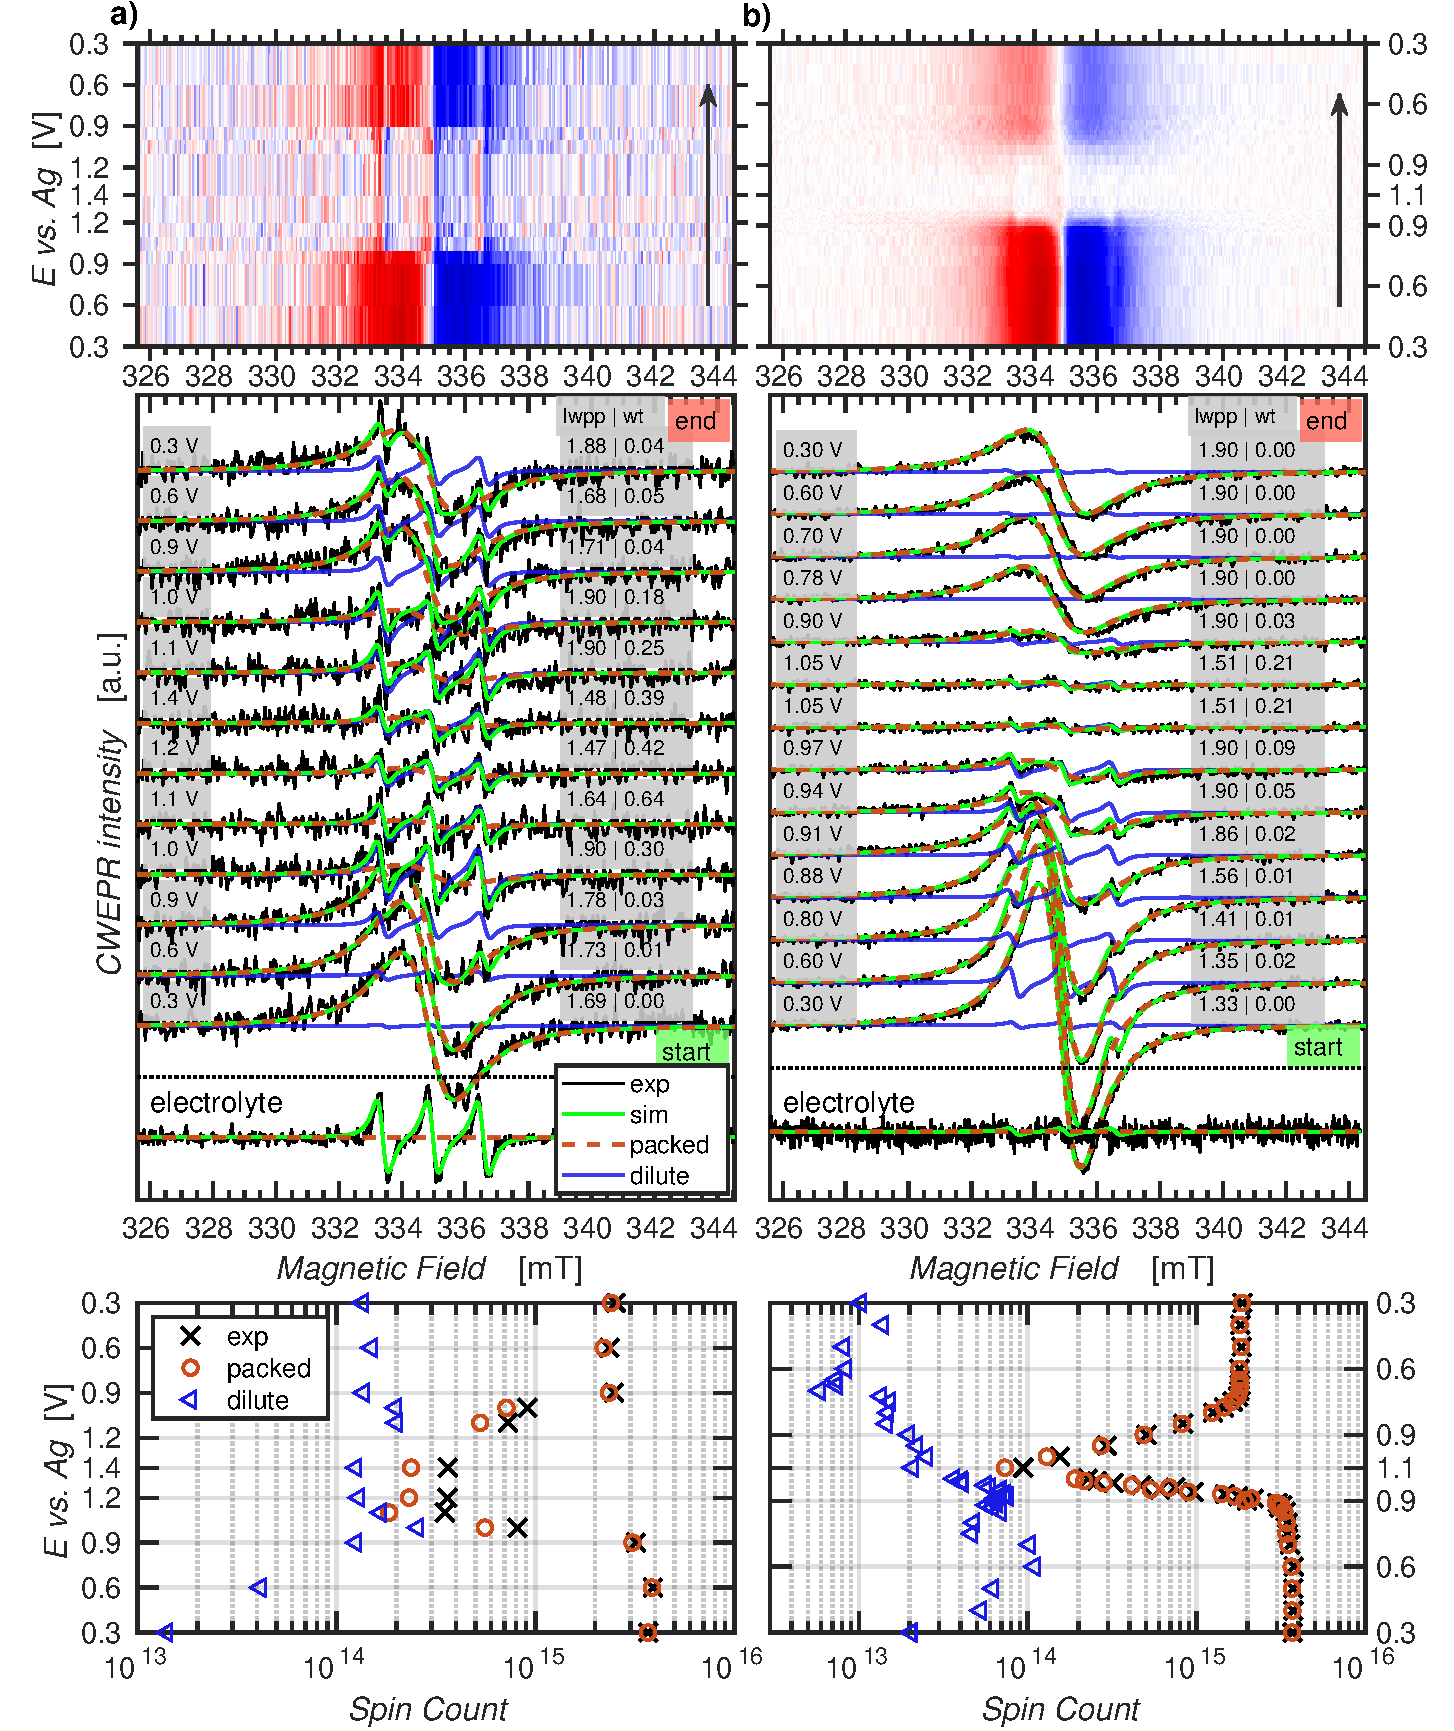
\includegraphics[width=1\textwidth]{./operando_epr/figures/degradation/operando_degradation_dits.pdf}
	\caption{Operando cwEPR spectra of two pDiTS electrochemical cells showing release of charge-bearing fragments upon the charge-discharge cycle.}
	\label{fig:operando_degradation}
\end{figure}

\begin{figure}[!h]
\center
	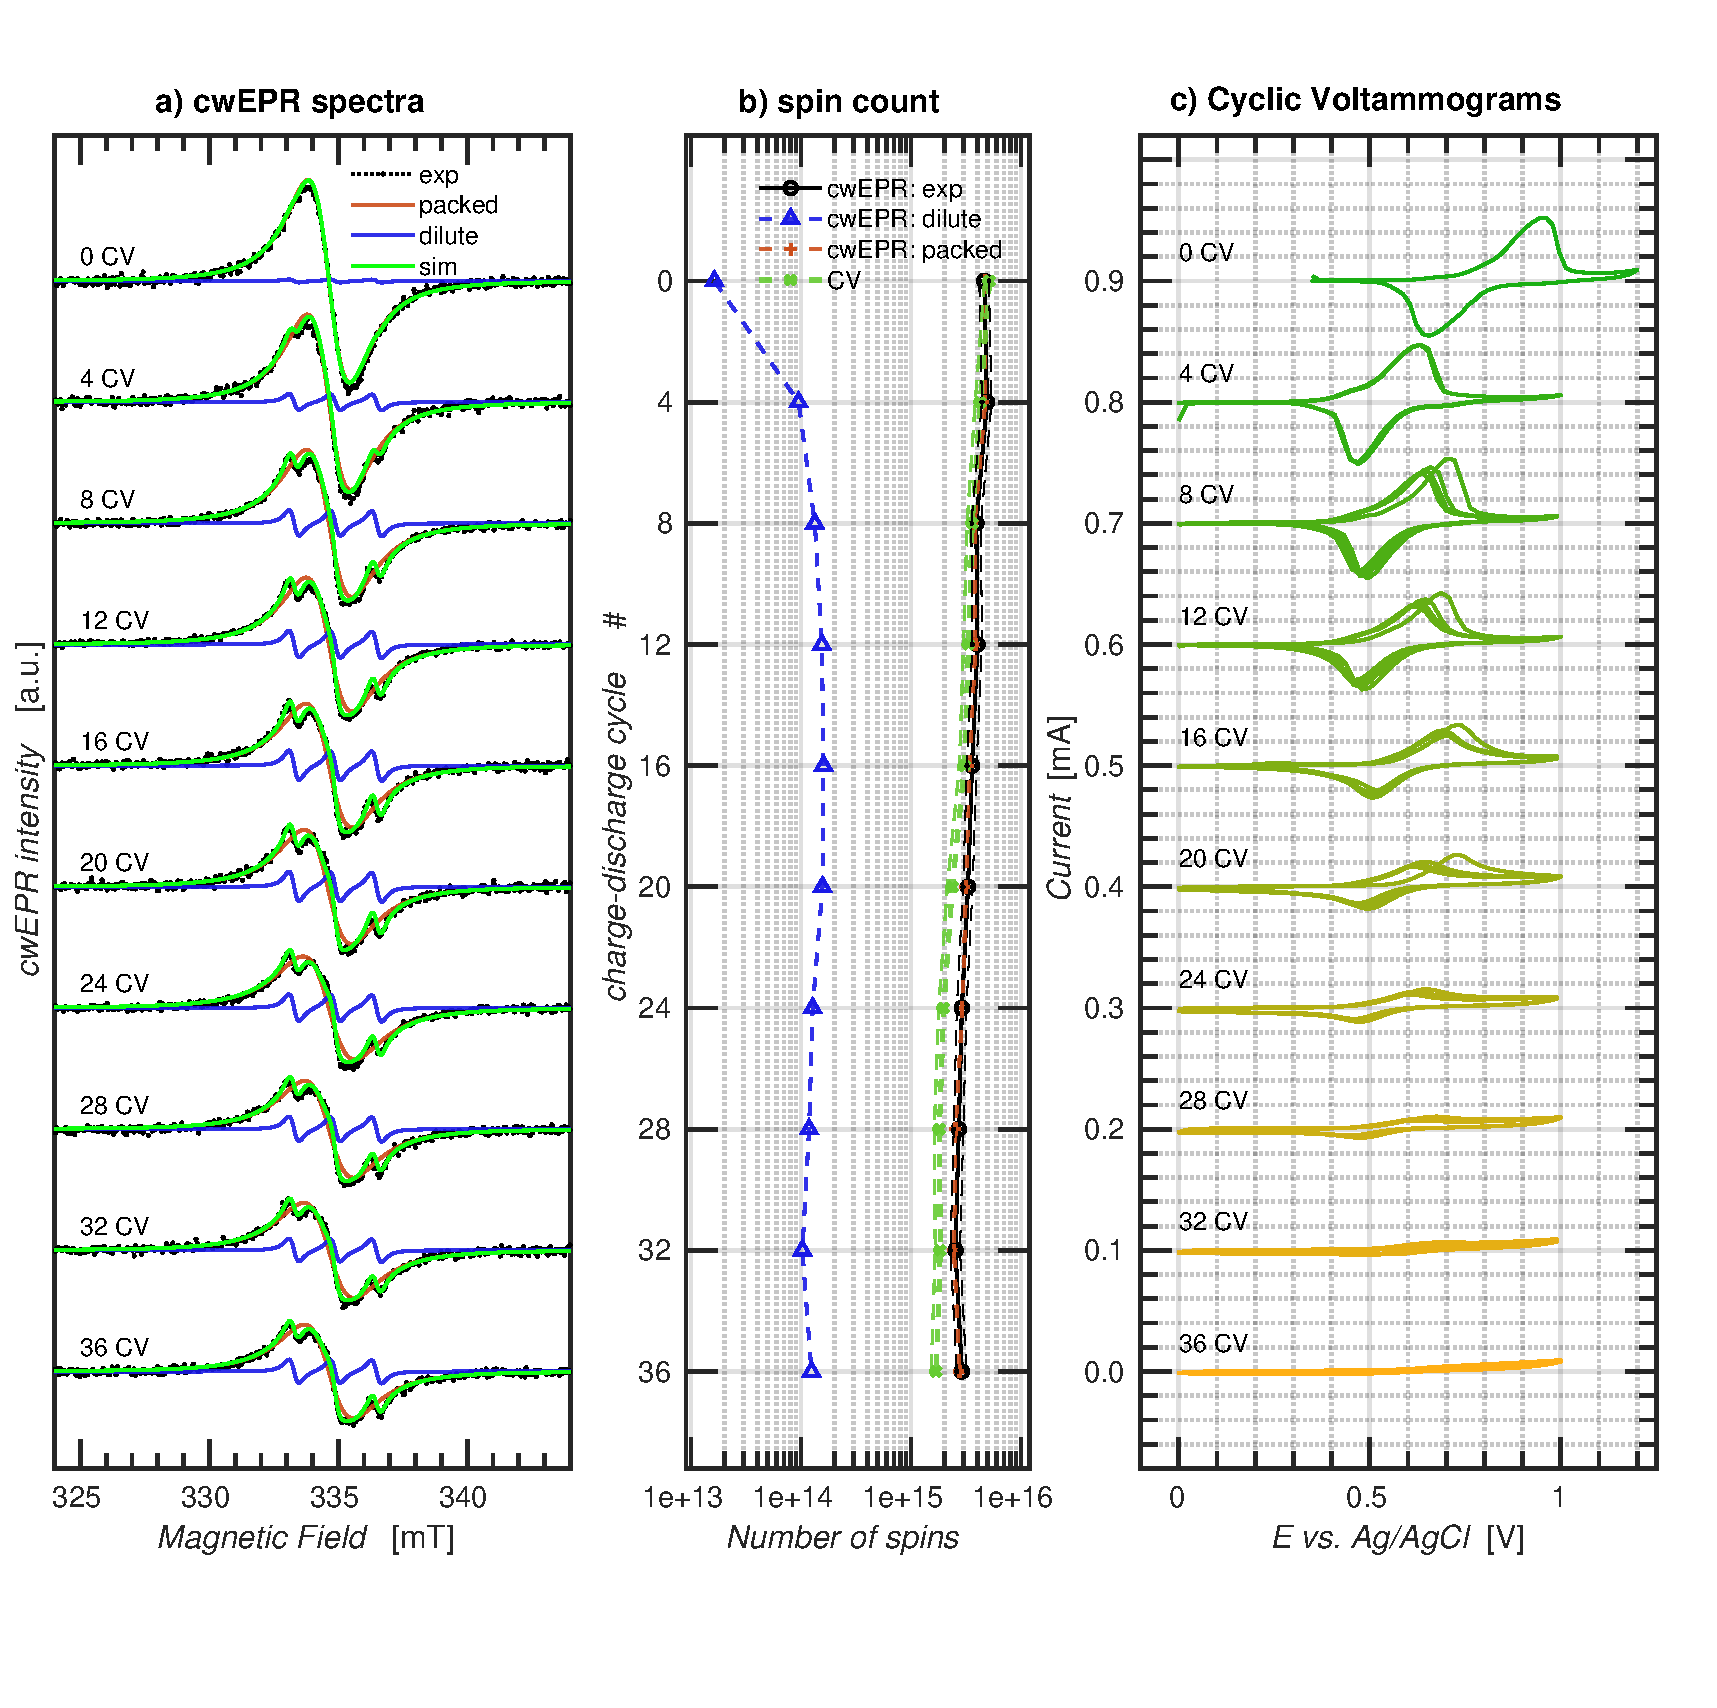
\includegraphics[width=1\textwidth]{./operando_epr/figures/degradation/repeated_cycling_degradation_dits.pdf}
	\caption{a): Evolution and component decomposition of cwEPR spectra for a tube-based, 150~CV p-DiTS ORB upon 36 charge-discharge cycles. b): Quantitative analysis of the separated spectral components. $\nu$ = 9.4$\,$GHz, Mod.~Amp:~0.5$\,$mT. Quantitative analysis of the CV curves. c): Cyclic voltammograms of the cell, recorded with respect to Ag/AgCl RE at a rate of 5~mV\,s\textsuperscript{-1} in between the EPR scans, in the modified tube inside the microwave resonator. The CV were taken at 5~mV\,s\textsuperscript{-1}, which is 10 times slower than the CV curves taken in the larger beaker, because limited amount of the electrolyte in the modified tube was found to strongly affect the shape and positions of the CV peaks at higher speeds of cycling.}
	\label{fig:repeated_cycling_degradation}
\end{figure}





\section{Monitoring of Self Discharge}
Organic Radical Batteries have a tendency to self-discharge, as the organic electrochemically active layer partially dissolves in polar electrolytes. Particularly for the TEMPO containing ORB, the dissolved, mobile TEMPO fragments serve as redox shuttles that carry the charge between the battery electrodes and cause a self discharge. The amount of unoxidized TEMPO$^\bullet$ shuttles can be measured with cwEPR spectroscopy as the mobile fragments have distinct spectra as compared to the fragments tightly packed in the electrode. Further in this subsection operando spectra of a TEMPO containing electrochemical cells are shown. Quantitative analysis of the released fragments during a charge-discharge cycle allows for a description of the self-discharge process in an ORB. The charge state of a battery is monitored with cwEPR and, additionally, with a potentiometric measurement to identify the self-discharge rate and to connect it with the concentration of diffusing redox shuttles. Figure~\ref{fig:self_discharge_DOM} represents a gradual change in the cwEPR intensity of a self-discharging tube-based cell with a pDiTS cathode. The cell was initially discharged to $V_{OC}=350$~mV and then charged to $V_{OC}=1300$~mV, at that point the minimal cwEPR intensity was registered. The cell was left under the open circuit condition. After $t=500$~s, the cwEPR signal of the cell has fully recovered, that corresponds to the complete reduction of the electrochemically active nitroxide radicals in the cathode film.

\begin{figure}[h]
\center
	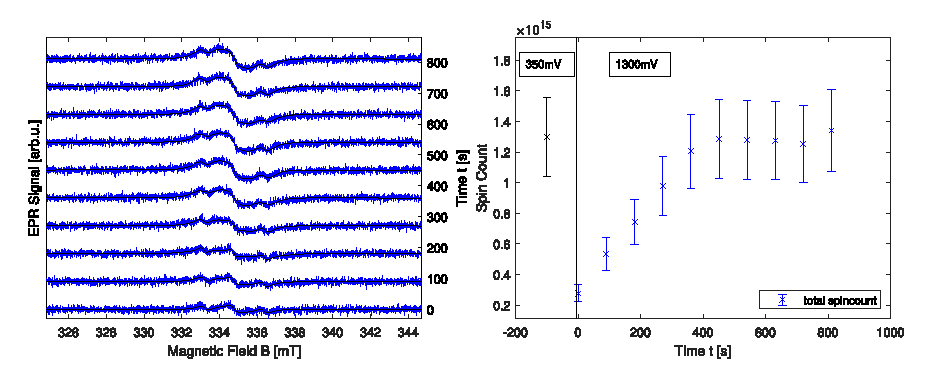
\includegraphics[width=1\textwidth]{./operando_epr/figures/self_discharge/DOM_DITS_SELF_DISCHARGE.pdf}
	\caption{cwEPR monitored self-discharge of a tube-based cell containing a pDiTS film made with 50 deposition cycles. Left: Development of the EPR spectra of the oxidised sample over time from bottom to top; Right: Development of the spincount of the oxidised sample over time and comparison to the reduced state.~\cite{DOM}}
	\label{fig:self_discharge_DOM}
\end{figure}





\begin{figure}[h]
\center
	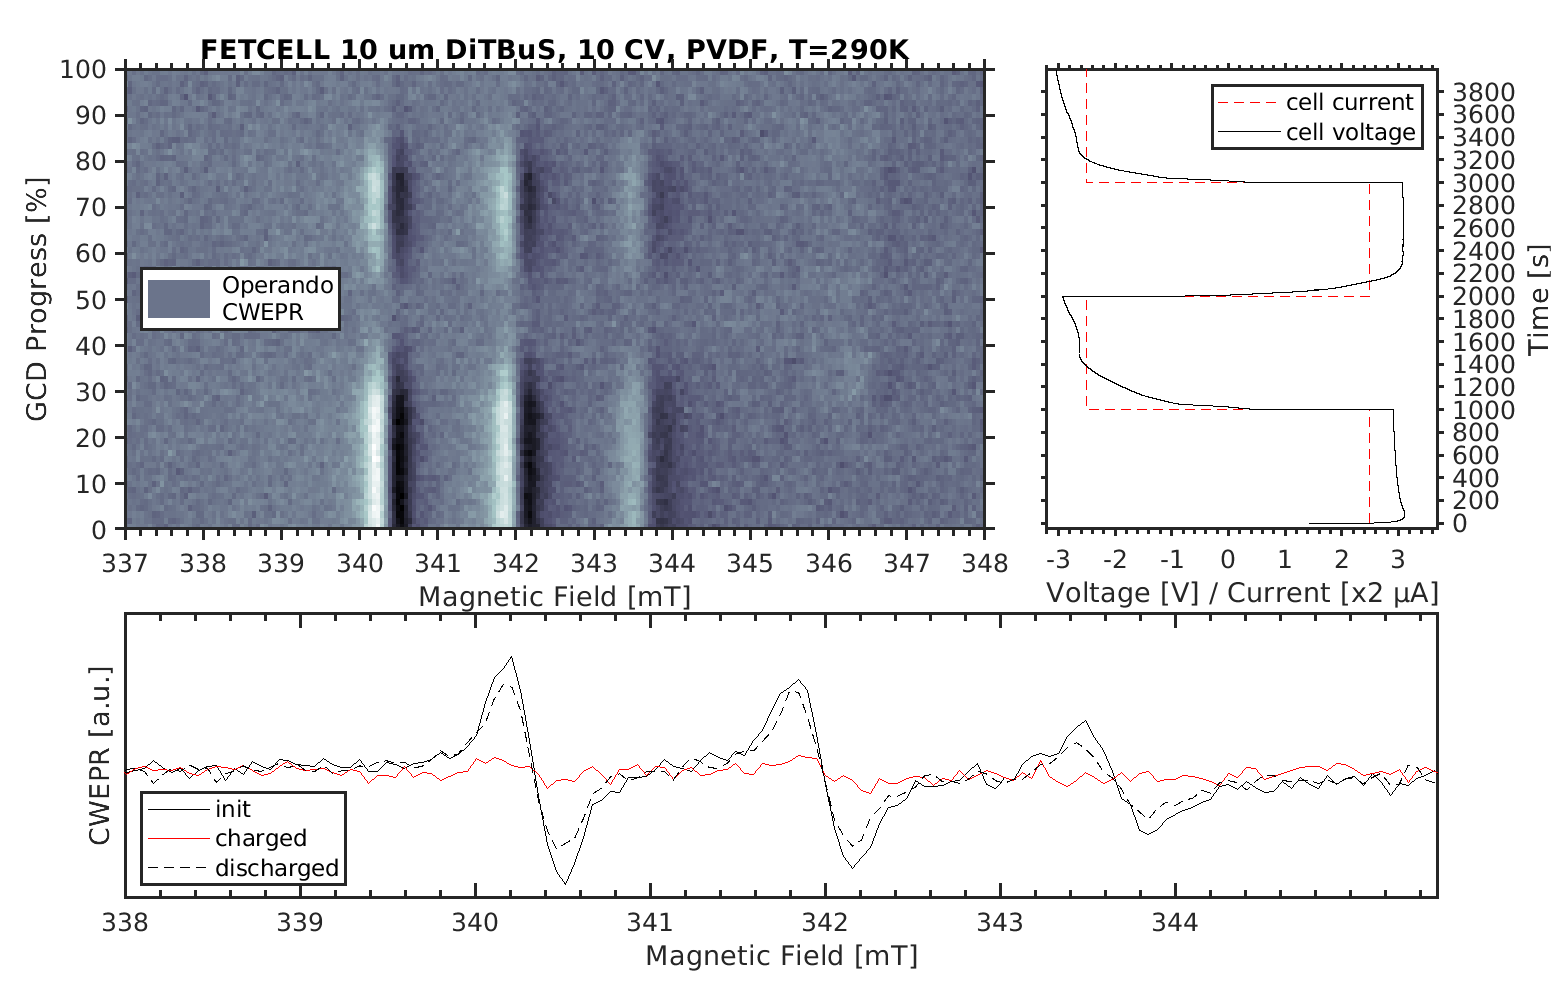
\includegraphics[width=1\textwidth]{./operando_epr/figures/solid/FET231114_5uA_RT.pdf}
	\caption{Operando cwEPR on an all-polymer organic radical battery made on a 5~$\muup$m grid with a PVDF/TFSI gel electrolyte.}
	\label{fig:operando_solid_battery}
\end{figure}

\section{Low Temperature Measurements}

\begin{figure}[h]
\center
	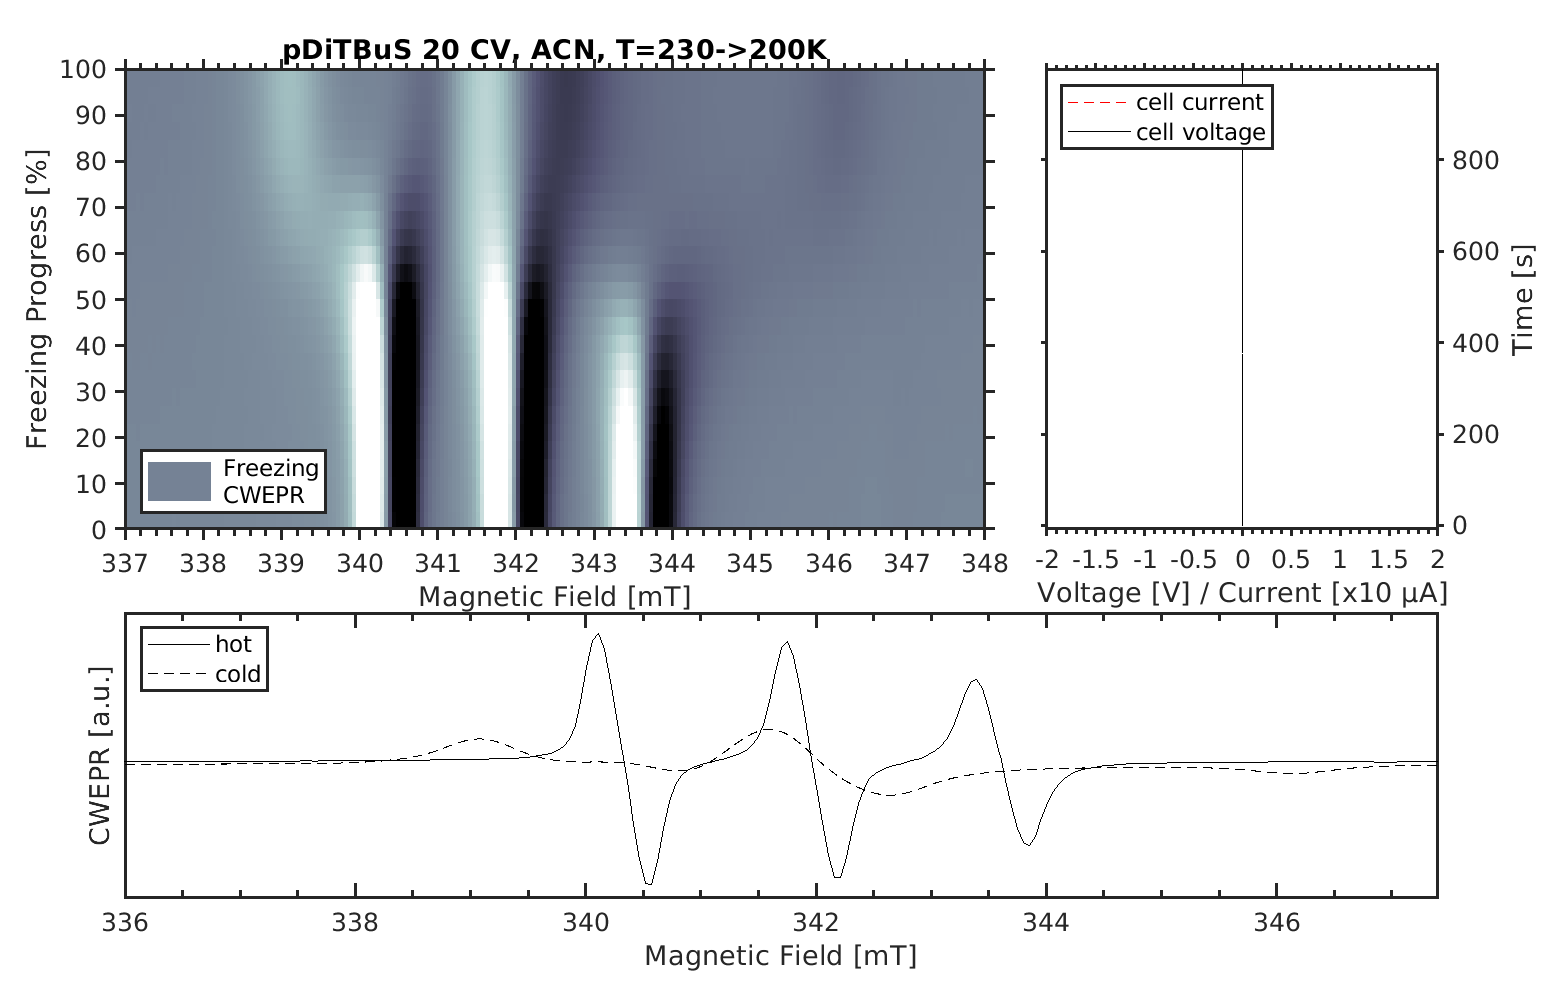
\includegraphics[width=1\textwidth]{./operando_epr/figures/CRYO/SANDWICH_FREEZING.pdf}
	\caption{Freezing a pDiTBuS cell}
	\label{fig:operando_cold_battery}
\end{figure}


\begin{figure}[h]
\center
	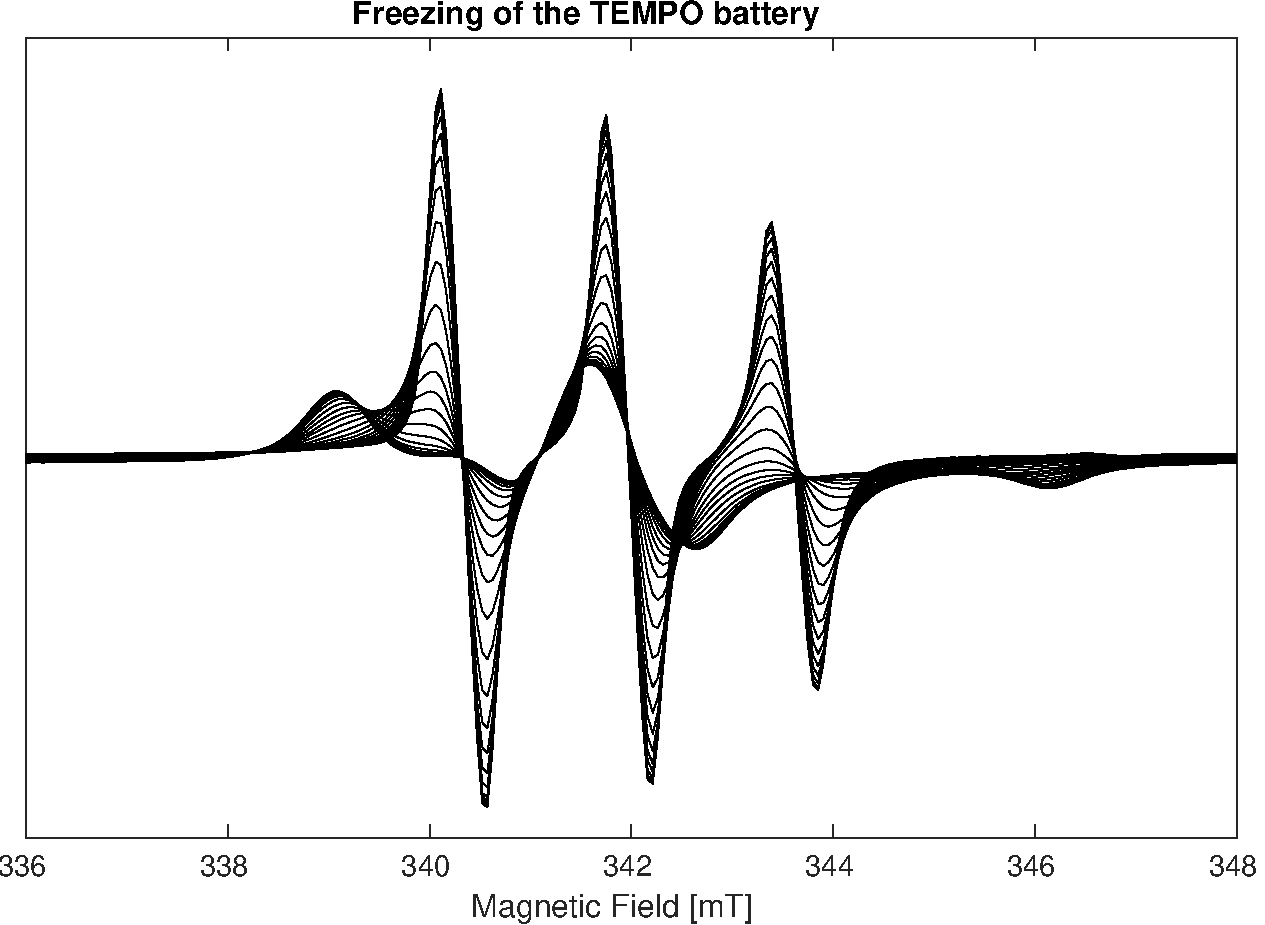
\includegraphics[width=1\textwidth]{./operando_epr/figures/CRYO/freezing_sandwich_230K_200K.pdf}
	\caption{Freezing a pDiTBuS cell}
	\label{fig:freezing_of_pditbus_battery_1D}
\end{figure}


\begin{figure}[h]
\center
	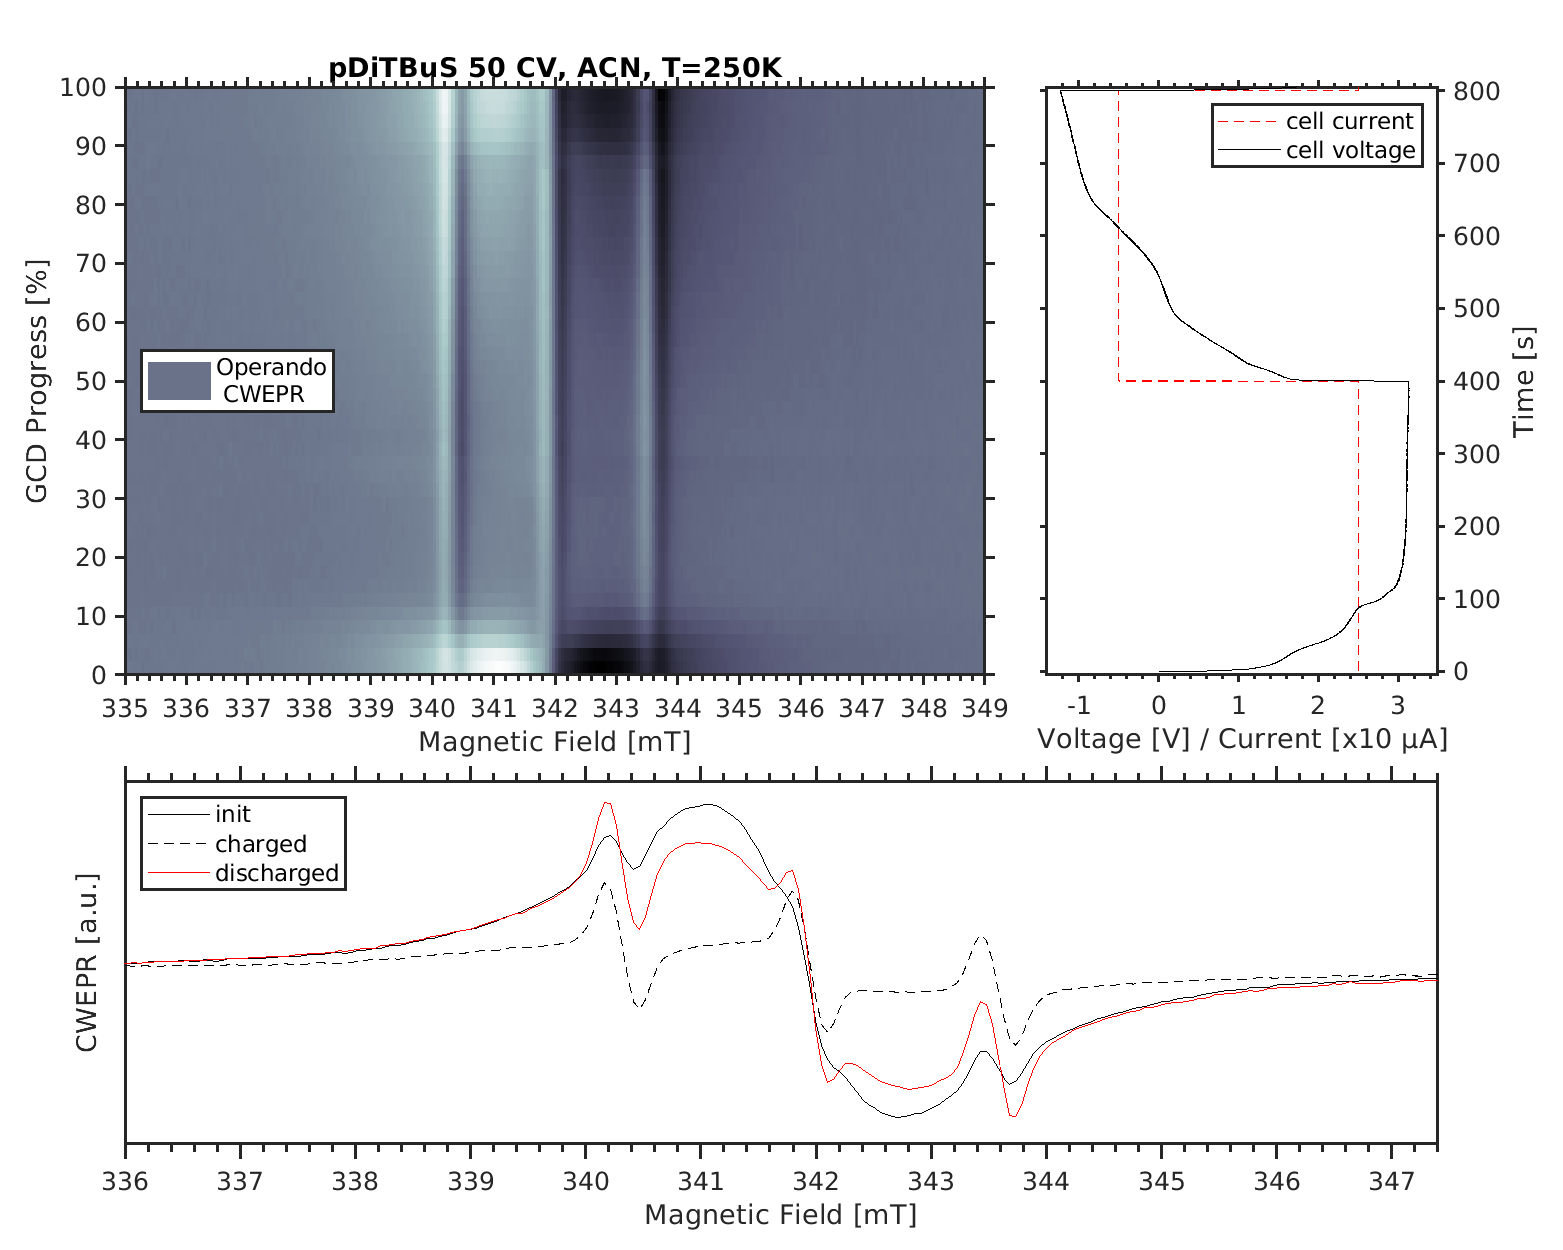
\includegraphics[width=1\textwidth]{./operando_epr/figures/slowcharge_231117_liquid_250K.pdf}
	\caption{XXX}
	\label{fig:operando_cold_cycle}
\end{figure}



\section{Pulsed EPR spectroscopy of a pDiTBuS Cathode Film}
\subsection{Pulsed EPR Spectra of TEMPOL solutions}
In a glassy, frozen solutions of TEMPOL, the distance between the TEMPO radicals is controlled by the concentration. With the increasing concentration, the relaxation times shorten significantly, as the distance between the radicals decreases, which intensifies the inter-spin interactions and leads to a faster in-plane dephasing of the excited spins.

\section{Pulsed EPR Spectroscopy of a charged pDiTBuS Cathode film}

\begin{figure}[h]
\center
	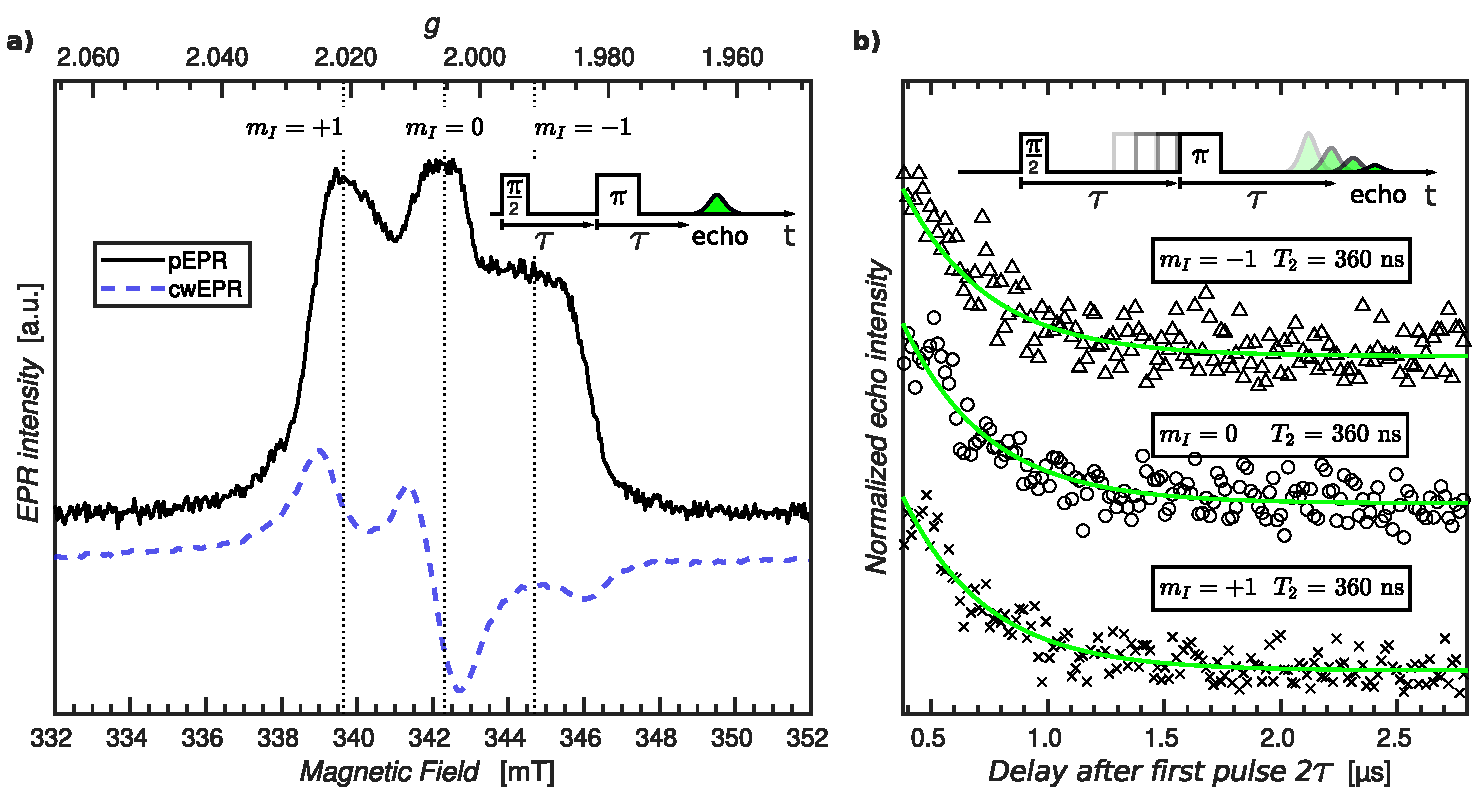
\includegraphics[width=1\textwidth]{./pulse/figures/SAW_Figure_8.pdf}
	\caption{X}
	\label{fig:FSE_vs_CW_DiTS_rel_times}
\end{figure}

\begin{figure}[h]
\center
	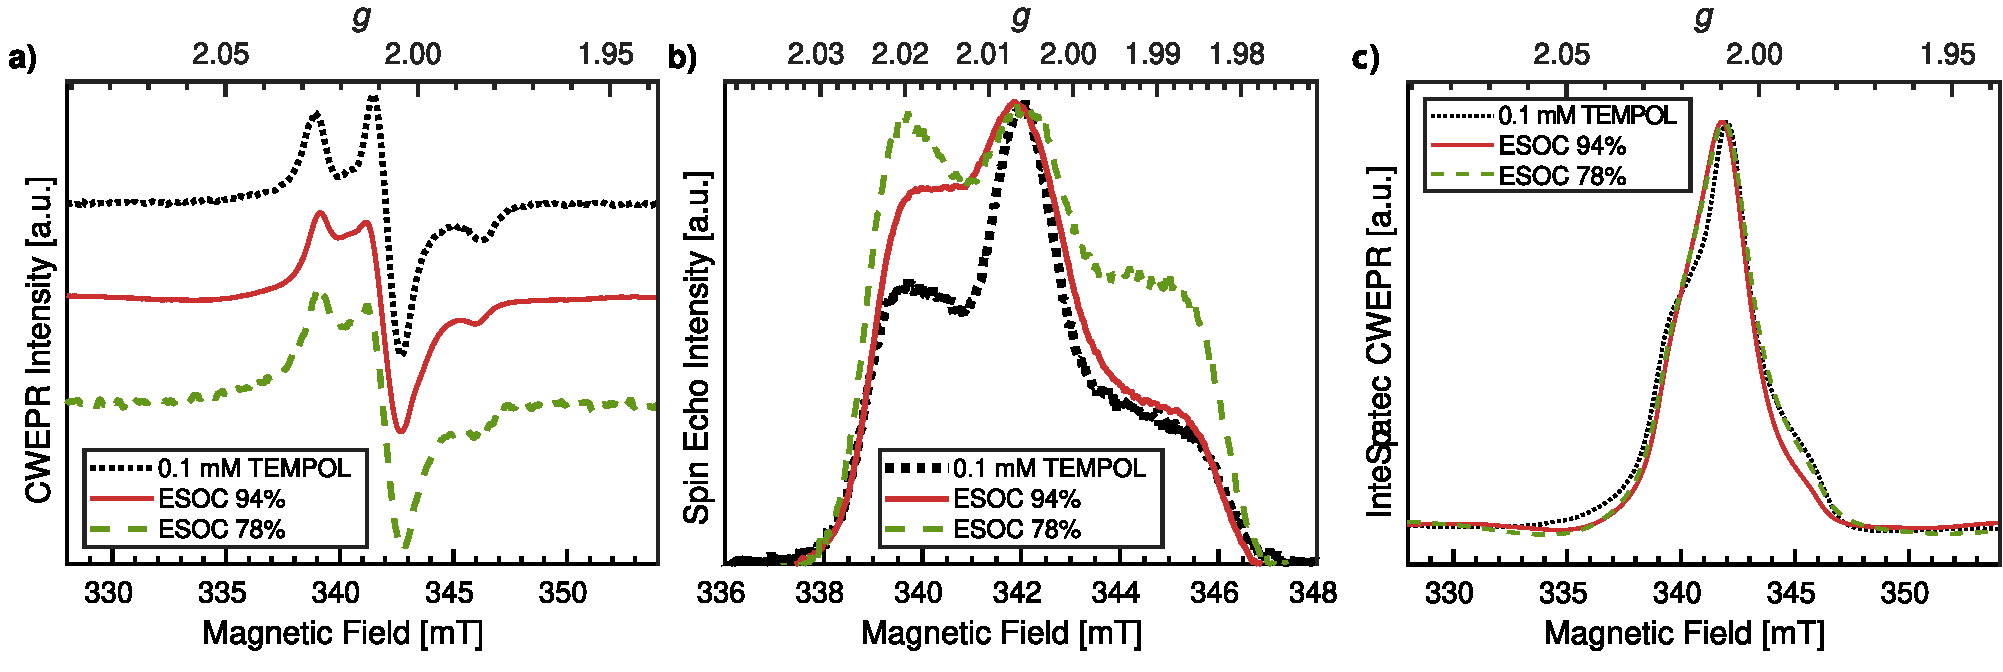
\includegraphics[width=1\textwidth]{./pulse/figures/Figure_3_INTS.pdf}
	\caption{a): cwEPR spectra for pDiTBuS charged to 95\% and 85\%, and for a frozen 0.1~\si{\milli\Molar}  solution of TEMPOL. Normalized intensities. Temperature 80~K. b): Corresponding \rs{pEPR} spectra measured at 5~K. Intensities scaled by the $m_I=0$ central peak. c): Integrated cwEPR intensities show similar spectral shapes. Temperature: 80~K, microwave frequency: 9.6~GHz, field modulation: 5~G at 100~kHz. ER~4118 X-MD5 dielectric ring resonator.}
	\label{fig:FSE_vs_CW_vs_INTS_DiTBuS}
\end{figure}



\begin{figure}[h]
\center
	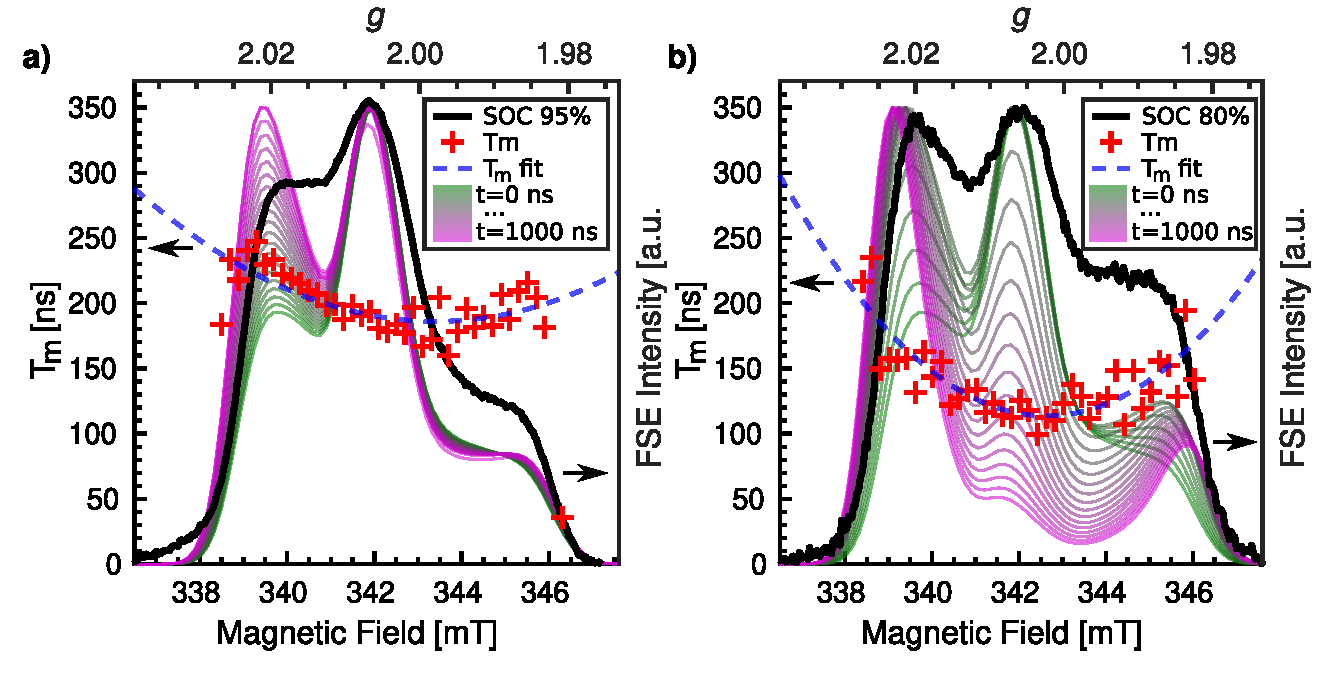
\includegraphics[width=1\textwidth]{./pulse/figures/Figure_6_maintext_col_MOD.pdf}
	\caption{X}
	\label{fig:FSE_reconstruction_with_T2}
\end{figure}



\subsection{Field Swept Echo of a charged pDiTBuS Cathode film}
\begin{figure}[h]
\center
	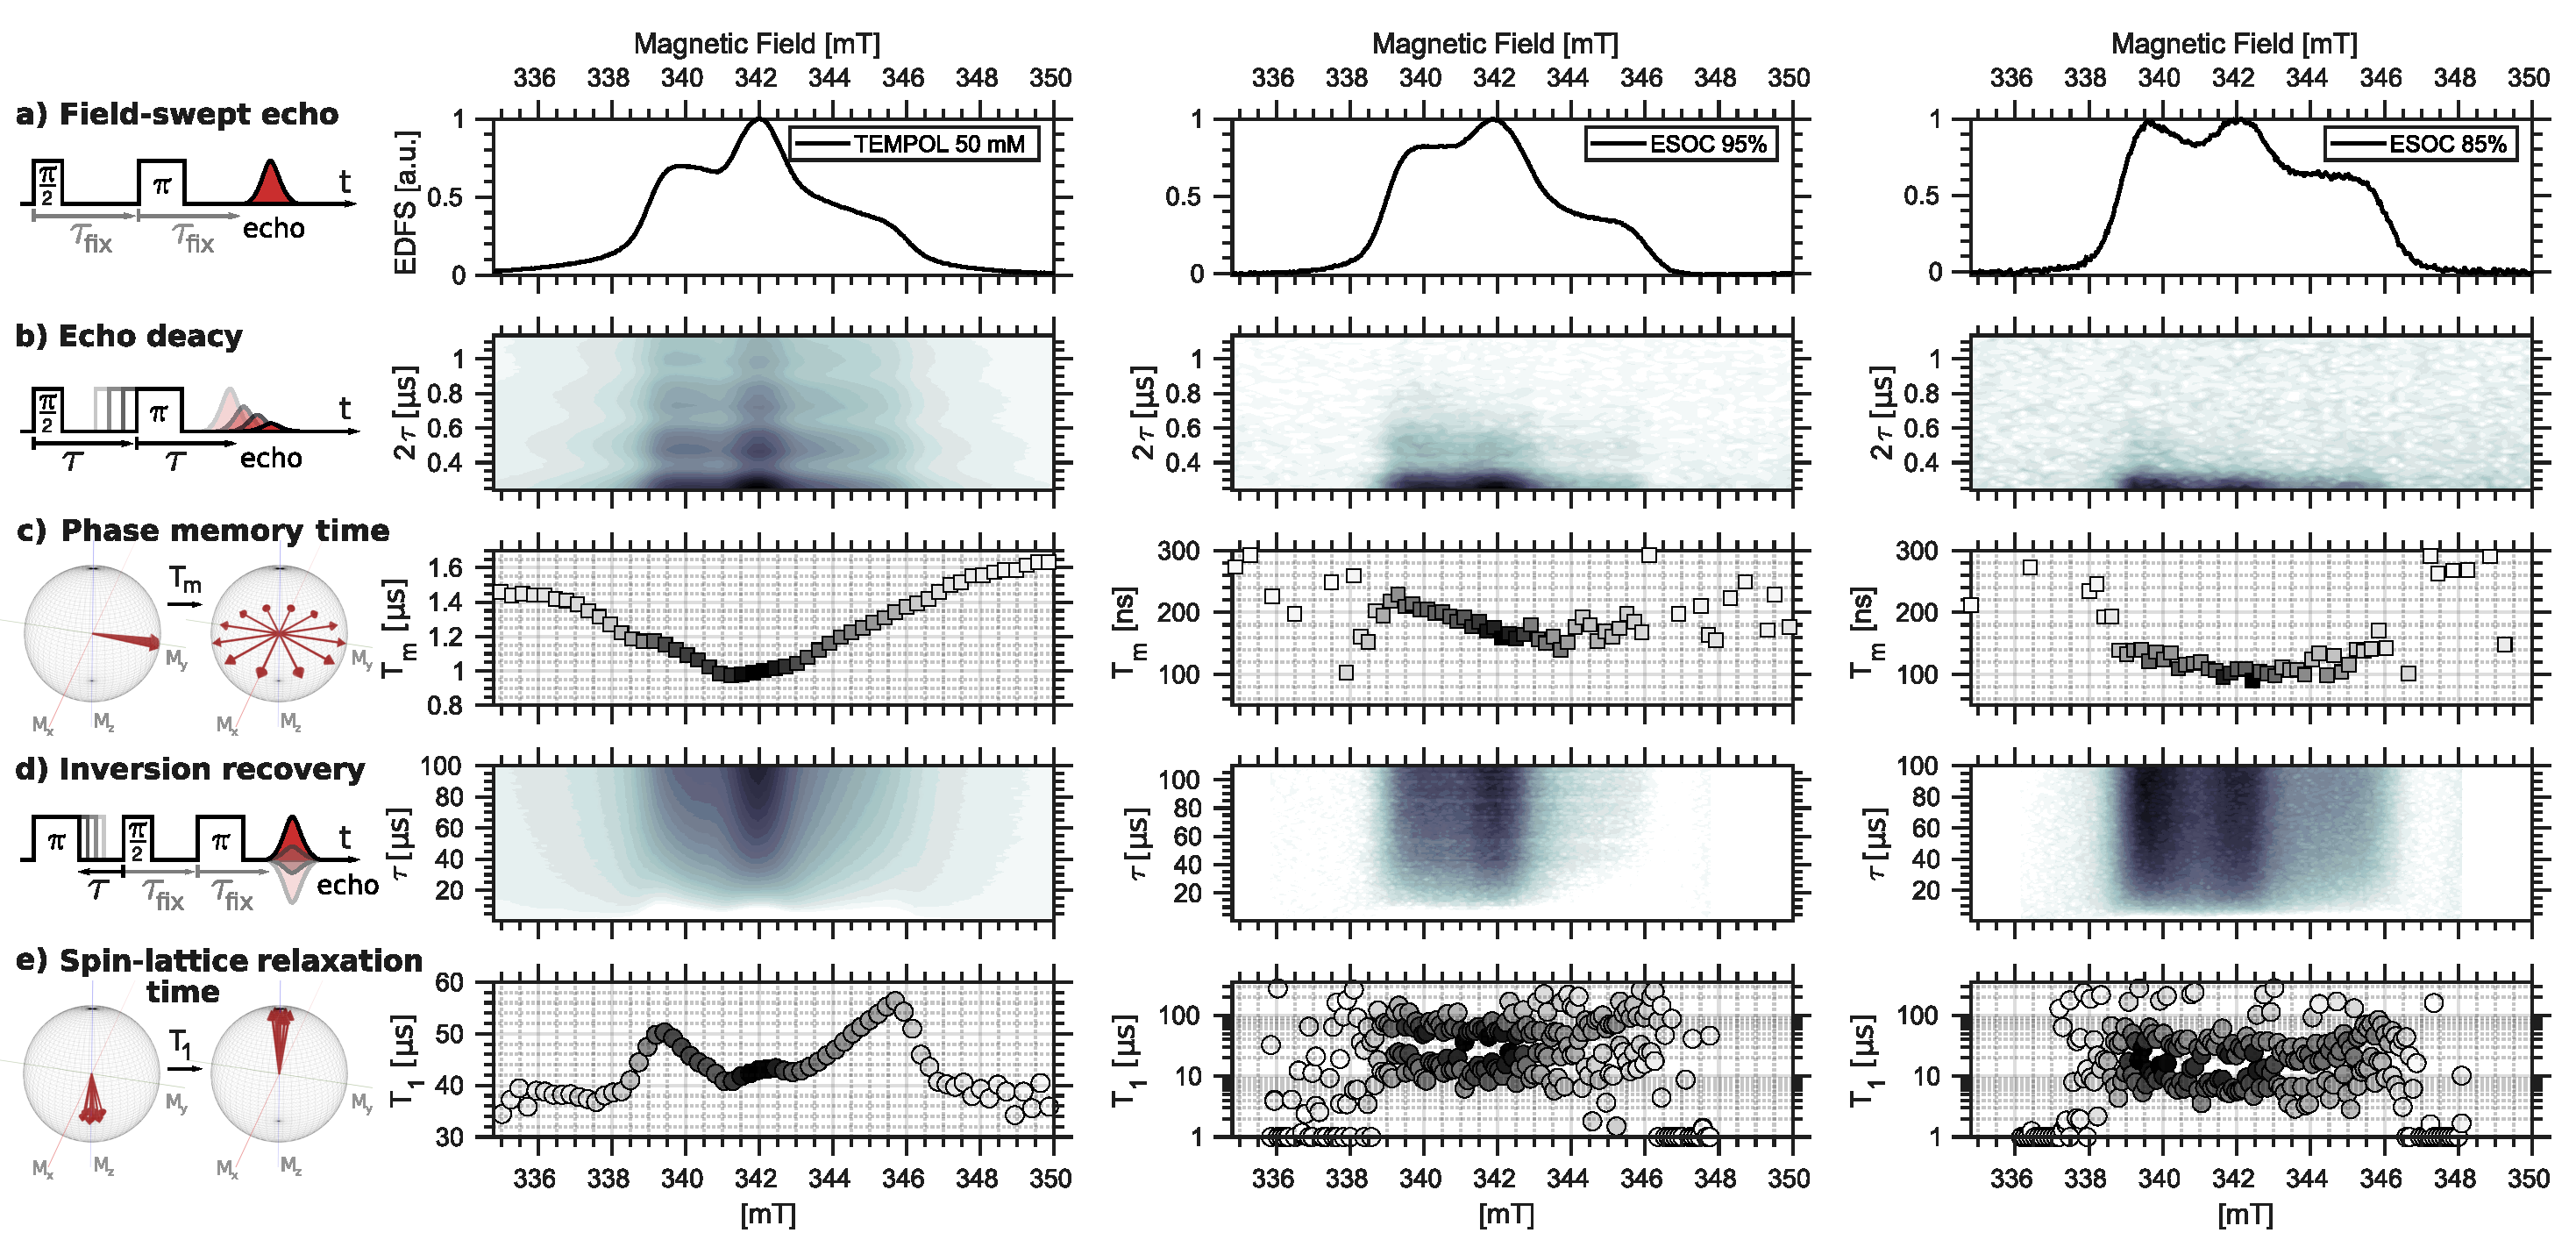
\includegraphics[width=1\textwidth]{./pulse/figures/FSE_DTBS_FSE_RELAX_T1Tm.pdf}
	\caption{XXX}
	\label{fig:Figure_FSE2}
\end{figure}

\subsection{Instantaneous Diffusion in Charged pDiTBuS}
\label{S:ID}

We have seen that \rs{the} ESOC has a strong influence on the shape of the EDFS spectra. Furthermore, the EDFS spectra of pDiTBuS are quite different from the reference spectrum of TEMPOL in a \rs{dilute} frozen solution.\\


In Section /// it is shown that in a densely packed radical system, as in a TEMPO-Salen cathode film, the phase memory time can be shorter than $T_m\leq100$~ns. That is, the spin echo is decaying by $e\approx3$ times at $t=100$~ns. The short phase memory time limits the duration of the pulse sequence at which the echo is detectable. For a $\pi/2-\tau-\pi-\tau-echo$ sequence, with a hardware limitation on $\tau\geq t_d\approx100$~ns, the shortest realizable pulse sequence becomes longer than $t>200$~ns. By this time, the spin echo decreases by $e^2\approx7$ times and may be comparable to noise. The limitations imposed by the finite $T_m$ and $t_d$ force one to use shorter microwave pulses. 
\par
A short microwave pulse may have a spectral width comparable to the width of the observed spectrum. According to the Fourier theorem, the spectral width of a pulse is inversely proportional to the pulse length: $\Delta\omega\sim 1/t_p$. A spectrum of a 100~ns long rectangular pulse shown in Figure /// is ///MHz wide (FWHM). 

\begin{figure}[h]
\center
	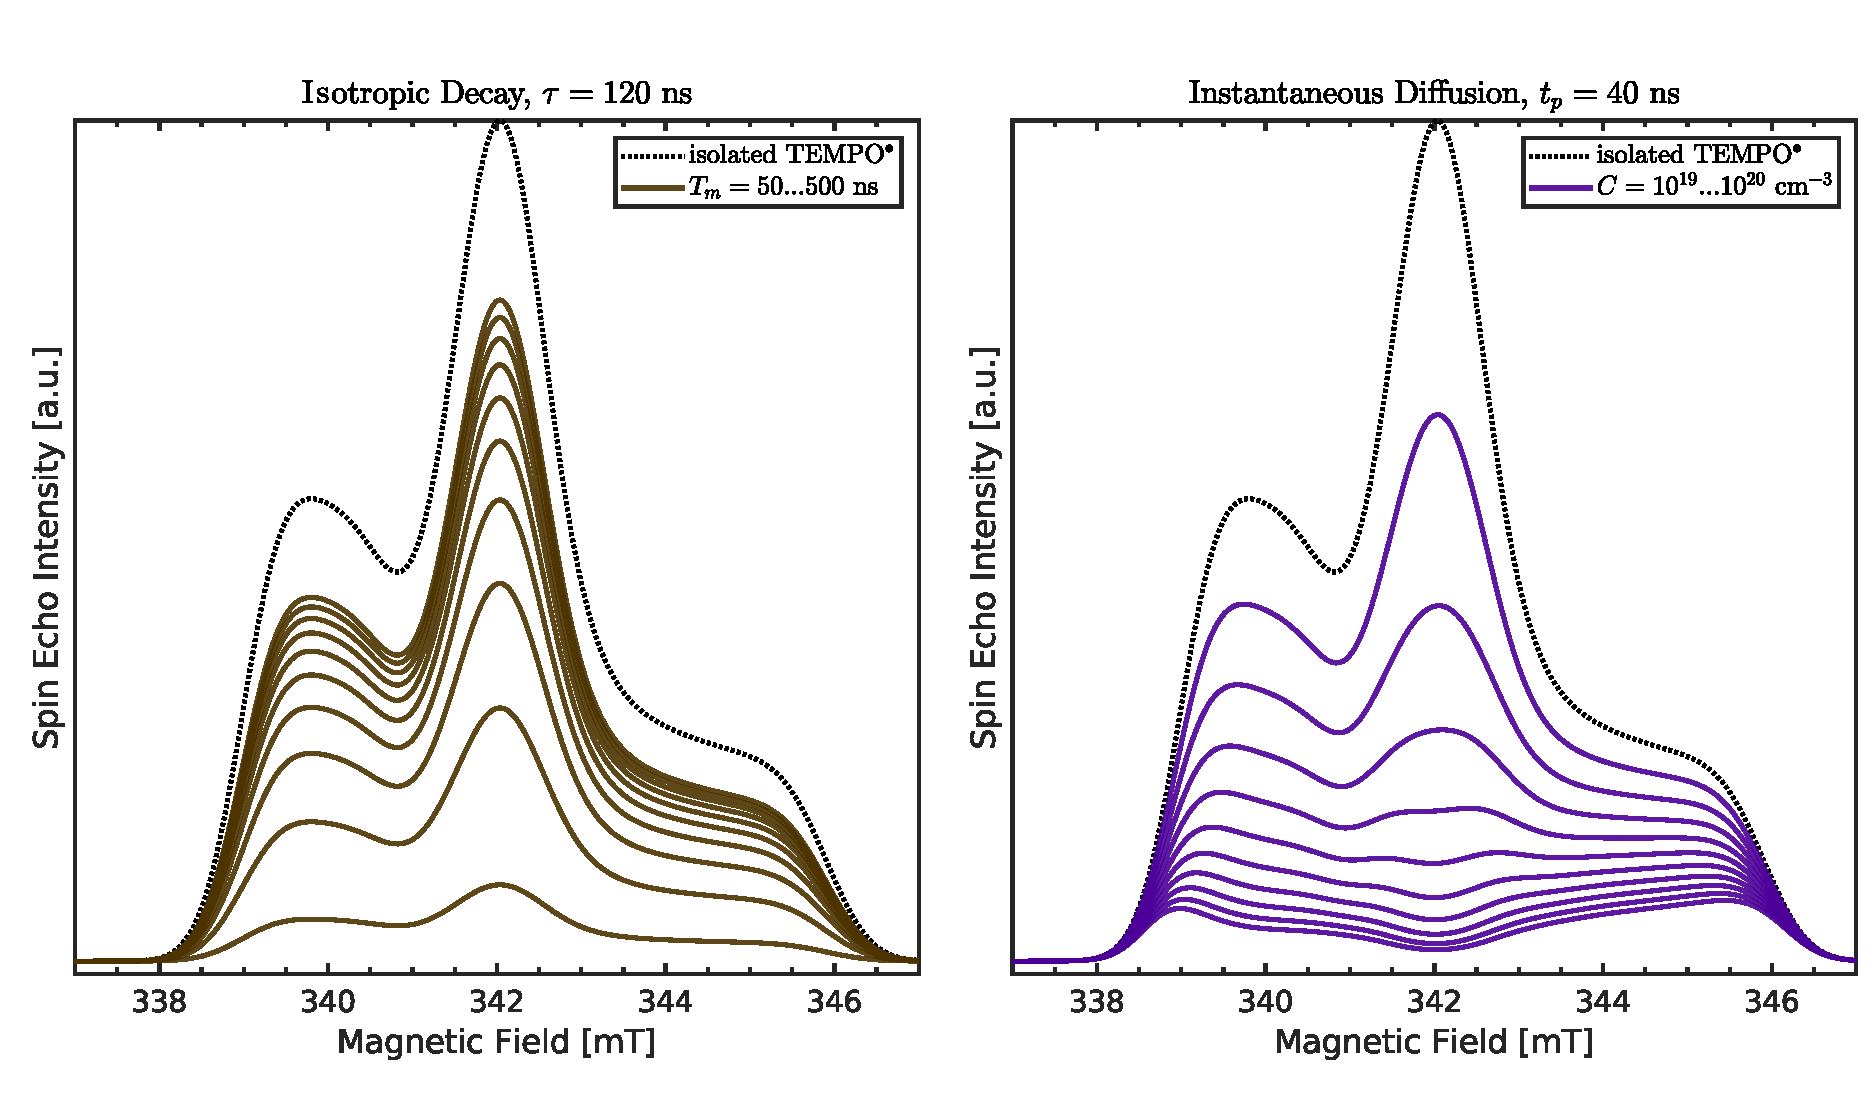
\includegraphics[width=1\textwidth]{./pulse/figures/FGMR/ID/ID_vs_ISO.pdf}
	\caption{Distortions of a nitroxide FSE spectrum caused by isotropic spin relaxation (left) and instantaneous diffusion (right).}
	\label{fig:iso_vs_id}
\end{figure}


















